\documentclass[11pt,twoside,a4paper]{book}

\usepackage[british]{babel}   % use UK hyphenation, etc.
\usepackage[T1]{fontenc}      % font printing stuff
\usepackage{ae,aecompl}       % scalable, non-bitmap fonts
\usepackage[pdftex]{graphicx} % enables graphics for pdf-latex
\usepackage{color}            % enables use of colour for text
\usepackage{subfig}           % enables subfigures
\usepackage{amsmath}          % the one and only AMS-Math
\usepackage{makeidx}          % creating an index
\usepackage{wrapfig}          % using floating figures

% ----------------------------------------------------------
% My own commands
% ----------------------------------------------------------
\newcommand{\mynote}[1]{\emph{\textbf{\textcolor{red}{#1}}}}
\newcommand{\ra}{$\rightarrow$}
\newcommand{\cmd}[1]{\texttt{#1}}
\newcommand{\ogs}{OpenGeoSys }
\newcommand{\bstart}[1]{\noindent\textbf{#1} }
\newcommand{\degree}{\ensuremath{^\circ}}


% ----------------------------------------------------------
% Typography
% ----------------------------------------------------------
\nonfrenchspacing             % grosser Abstand nach Satzende
\widowpenalty 10000           % Keine Hurenkinder
\displaywidowpenalty 10000    % Keine Hurenkinder (Formeln)
\clubpenalty 10000            % Keine Schusterjungen


% ----------------------------------------------------------
% Headers
% ----------------------------------------------------------
\usepackage{fancyhdr}         % formating page headers

\renewcommand{\headrulewidth}{0.4pt}
\renewcommand{\footrulewidth}{0pt}
\fancyhead{} \fancyfoot{}
\fancyhead[RE]{The OpenGeoSys Data Explorer}
%\fancyhead[RE]{\nouppercase{\leftmark}}
\fancyhead[LO]{\nouppercase{\leftmark}}
\fancyhead[LE,RO]{\thepage}


% ----------------------------------------------------------
% Hyperref Options
% MUSS AM SCHLUSS DER PRAEAMBEL STEHEN!
% ----------------------------------------------------------
\usepackage{hyperref}         % references and links within the document

\hypersetup{
  pdftitle={OGS Data Explorer - User Manual},
  pdfsubject={Manual},
  pdfauthor={Karsten Rink},
  pdfcreator={LaTeX2e},
  plainpages=false,           % For problems with page referencing
  hypertexnames=false,        % For handling subfigures correctly
  bookmarks=true,             % I want bookmarks
  bookmarksnumbered=false,    % Include the section numbers in the list
  bookmarksopen=true,         % In the list, display highest level only
  bookmarksopenlevel=3,       % Display three levels of bookmarks
  pdfpagemode=UseNone,        % Fit screen (or "`FullScreen"')
  pdfstartview=Fit,
  pdfborder=0,                % I don't want those silly boxes
  breaklinks=true,            % Allow breaks in links
  colorlinks=false            % Don't change coloring of links
}


% ----------------------------------------------------------
% Document description
% ----------------------------------------------------------
\title{{\LARGE OpenGeoSys Data Explorer}\\[0.5em] Manual}
\author{Karsten Rink}
\graphicspath{{pics/}}
\setlength{\fboxsep}{0mm}
\linespread{1.10}

\makeindex

\hyphenation{know-ledge}

% ----------------------------------------------------------
% Start of document
% ----------------------------------------------------------
\begin{document}

\pagestyle{empty}
\maketitle
\newpage

\vspace*{12cm}
\begin{tabbing}
\hspace*{6cm}\=aa\kill
\begin{minipage}[t]{0.62\textwidth}
\noindent This manual has been compiled based on the \ogs Data Explorer 6 beta \\
(as of October 2013).\\
\\
This document as well as its sources are published under Creative Commons Attribution-Noncommercial-Share Alike 3.0 Un\-por\-ted License. For more information go to \url{http://creativecommons.org/licenses/by-nc-sa/3.0/}. \\
\\
\noindent Special thanks to Lars Bilke and Thomas Fischer and everyone else helping with the development of the software.
\end{minipage}
\> \\
\end{tabbing}

\newpage

\tableofcontents

\cleardoublepage

\pagestyle{fancy}

\chapter{Introduction}

This manual has been written to give a quick overview over the functionality of the \ogsde{}. Existing functionality is explained and typical workflows are detailed step by step.

\bigskip

\ogs{} (formerly Rockflow) is an open-source programme for the simulation of (coupled) thermal, hydrological, mechanical and chemical processes. Over various iterations the software is about $20$ years old and compiles a large amount of functionality, interfaces and numerical solvers. It is, however, a command line tool. Therefore, it is difficult to get a feeling for the data that is handled by the programme and input data as well as simulation results cannot be directly verified without the help of other programmes.

The \ogsde{} is a graphical user interface (GUI) has been developed to fill that gap and provide the necessary functionality for the visualisation of such data. It employs the same basic data structures as the command line tool and thus complements \ogs{} by giving the user a way to visually assess the data and see possible artefacts, inconsistencies between data sets or missing information.

However, it is important to keep in mind that the \ogsde{} is not yet \emph{not} a fully developed programme with a defined scope of functionality. Features are constantly being added and while everyone is making an effort to keep things as straightforward and robust as possible, it can be difficult to find out what the software is currently capable of and how exactly things need to be done.

This manual will give an overview of features implemented in the programme, how things work and what possible problems might occur in certain situations. For more information on \ogs{} itself check out the \ogs{}-website\footnote{\url{http://www.opengeosys.org}}.\index{OGS Website}

It is also highly recommended to always use the latest version of the  of the \de{} to be able to make use of recently implemented functionality, bug fixes, etc. The programme is available from the OGS-website or from the Github repository at \url{https://github.com/ufz/ogs}.

\section{User Interface Components}

\begin{figure}[tb]
\begin{center}
\includegraphics[width=0.99\linewidth]{gui}
\caption{The graphical user interface of the \ogsde{}.}
\label{fig:gui}
\end{center}
\end{figure}

Within this manual a number of specific terms will be used to refer to certain components of the \ogsde{}-framework. This section will give an overview of these components, such that readers will be able to follow the instructions in the following chapters.

Figure \ref{fig:gui} shows an illustration of the GUI of the \ogsde{}. The three basic parts of the user interface are marked as ``Data View'', ``Render Window'' and ``Visualisation Pipeline''. These elements and the information they contain are explained in detail in section \ref{datavisualisation} and these names will appear again and again in this manual so it is important to recognise which parts of the graphical user interface they specify. Additional windows might pop up from time to time for data that is not suitable for 3D visualisation, such as time series sensor data or borehole stratigraphies.

\ogs is written in the C++ programming language. As many other programming languages it allows the developer to add so-called libraries that define a certain set of functionality. This means a programmer does not need to implement every function provided by a programme himself but instead can depend on functionality provided by the library. The \de{} makes use of a number of such libraries. The two most important ones are called Qt\footnote{\url{http://qt.nokia.com}} and VTK\footnote{\url{http://www.vtk.org}}.

Qt\index{Qt} is a library mainly providing functionality for a user interface, i.e. the definition of windows, dialogues and everything you expect to see in there, such as buttons, lists, menus, etc. Qt offers a lot more than that, the interested reader is referred to the Qt-website for more information. Elements of the \ogsde{} that make use of Qt are for instance the ``Data View'' or the windows displaying diagrams or borehole stratigraphies.

VTK\index{VTK} (``\textbf{V}isualisation \textbf{T}ool\textbf{k}it'') is a graphics library which can be employed for the visualisation of objects in 3D. It also includes functionality to read and write these 3D objects from and to files. These VTK-files and can also be read and written by the \ogsde{} as well as other software supporting VTK, including ParaView\footnote{http://www.paraview.org}\index{ParaView} or OpenFOAM\footnote{http://www.openfoam.com}\index{OpenFOAM}. The ``Render Window'' of the \de{} and anything that is displayed within has been constructed using VTK.

\section{OGS Download and Installation}

The \ogsde{} is available for $64$-bit \emph{Ubuntu-} and \emph{Mac OS X} systems as well as for $32$- or $64$-bit \emph{Windows} operation systems, respectively. It is recommended to download the $64$-bit version for 64-bit \emph{Windows.} The binary files needed to run the programme can be found at \url{https://www.opengeosys.org/ogs-5/}. The console version of the \ogs{} simulation software is available on the same website.\index{Download}

To use \ogs{} or the \de{} under \emph{Windows,} it is necessary to additionally download and install the free ``Visual Studio Redistributable''-package\index{Redistributable Package} from \emph{Microsoft.} It is available directly on the \ogs{} download page. The downloaded version of this package needs to be for the same architecture (i.e. 32- or 64-bit) as the downloaded version for the \de{}. Without this additional package, DLL-related error messages will be displayed on start-up.

Once all necessary packages are installed, the \de{} needs only to be extracted from the downloaded zip-files to any directory and can be run instantly. For \emph{Windows,} start \cmd{ogs-gui.exe} to run the GUI. Using \emph{Ubuntu} or \emph{Mac OS X,} the programme can be started by calling \cmd{./ogs-gui}.\index{Installation}

\subsection*{Additional Software}

For be able to use the full functionality of the \de{}, two additional utilities are needed. Both are \emph{not} strictly required, but the functionality for creating finite element meshes described in this tutorial will not work without these additional programmes.

The first programme is the finite element mesh generator \emph{GMSH.}\index{GMSH} It is freely available and required for creating domain discretisations (meshes) from geometry (see section \ref{meshcreation}). The software is available for \emph{Linux, Mac OS X} and \emph{Windows} and installation files can be found at \url{http://geuz.org/gmsh/}. The second utility is the \emph{TetGen}\index{TetGen} finite mesh generator\footnote{The source code for \emph{TetGen} is available from the Weierstrass Institute Berlin at \url{http://wias-berlin.de/software/tetgen/}. A binary file is available from the UFZ GitHub reprository at \url{https://github.com/ufz/tetgen}.}. It is required for creating 3D tetrahedral meshes from 2D meshes as described in section \ref{meshondemmapping}.

While \emph{TetGen} is used only indirectly by the \de{}, GMSH can be directly controlled via user interface dialogues. Therefore, it is recommended on first start-up of  the \emph{Data Explorer} to set the location of this programme. This is done by selecting \cmd{Settings \ra Data Explorer Settings...}. A new dialogue will open where the location can be specified.

\section{Source Code Availability}

As mentioned before, \emph{OpenGeoSys} is a cross-platform open-source software. If \emph{OGS} should be run on an operating system where no binary files are available, it is still possible to download and compile the source code.

All necessary files as well as the manual may be found on GitHub at \url{https://github.com/ufz/ogs}. A developer guide detailing everything necessary for compilation can be found at \url{http://docs.opengeosys.org}. You are also invited to join further development of the software if you are inclined to do so.

\emph{OpenGeoSys} and the \emph{Data Explorer} are available under BSD license, i.e.~both are free for non-commercial use as as long as  the \emph{OpenGeoSys Community} is referenced as the developer of the software. The exact conditions of use can be found in the file \cmd{LICENSE.txt} on the GitHub-repository.






\chapter{Working with the Data Explorer}

\section{Loading data}

\subsection{Data Types}
\label{datatypes}

\ogs distinguishes between different types of data such as geometry, meshes and process-dependent data. The \emph{Data View} of the Data Explorer reflects this distinction by separating all the data loaded into the programme into one of the four tabs of the data view:

\begin{figure}[tb]
\begin{center}
\includegraphics[width=0.95\linewidth]{elementtypes}
\caption{Mesh element types supported by \ogs.}
\label{fig:elements}
\end{center}
\end{figure}

\begin{itemize}
\item \textbf{Geometrical data} includes points, polylines and surfaces. To be more specific, points include any location in 3D space by giving an $x$, $y$ and $z$ coordinate. Lines are a ordered list of points, the can closed to represent polygons by specifying the first and last point of the line to be identical. Finally, surfaces are composed of triangles, which in turn are consisting of three points. To decide which direction a triangle is facing, points are given in counter-clockwise order on the ``up-side''.\index{Geometry}
\item \textbf{Meshes} are domain discretisations in 2D or 3D. Each mesh contains a set of nodes (points) as well as a set of elements defined by a subset of these nodes. A mesh may contain different kinds of elements. OGS supports the following element types\index{Element types}: lines, triangles, quadrilaterals, tetrahedra, hexahedra, pyramids, prisms. See figure \ref{fig:elements} for example elements and node numbering.\\
    Meshes are often classified into structured or unstructured meshes. Note, that \ogs treats all meshes as unstructured, independent of their actual structure.\index{Meshes}
\item \textbf{Stations} include observation sites of data loggers or boreholes. This data differs from geometry as it contains additional information for each object such as stratigraphic information for boreholes or time series data for data loggers. Within the Data Explorer this data is visualised in a different way.\index{Observation Sites}
\item \textbf{Modelling data} supported by the data explorer is currently only a listing of processes with their primary variables as well as initial- and boundary conditions. These conditions can be applied to geometrical objects or mesh nodes and these will also be visualised in the render window.\index{FEM Conditions}
\end{itemize}


\subsection{Native File Formats}
\label{nativefileformats}
\index{File formats}

\ogs has a large number of native file formats for storing geometrical data, meshes, processes, FEM conditions (such as boundary conditions) and material properties (e.g. fluid properties) and many more.

Not all of them can be loaded into the user interface since not all of them contain data that can be visualised. Things are additionally made difficult as the file standards for the programm are currently changed from GeoSys4 legacy files in ASCII format to XML files\footnote{http://www.w3.org/XML/}. For this reason there exists -- at least at the time of this writing -- two file standards for certain kinds of data. Currently the legacy files can still be read for the most part but not be written anymore. There is also a small file converter tool deployed with the OGS6 package (see section \ref{FileConverter})

You can open all native OGS files by clicking \cmd{File\ra Open...}\index{Loading geometry}\index{Loading meshes}. As an alternative, files can also be opened by clicking the folder icon in the respective Data View tab. However, this will only allow to open files relevant for this specific tab, i.e. if the folder-icon in the \emph{Geometry}-tab is pressed, you will only be allowed to open geometry-data. Please note that all files \emph{must} have the correct file extension for the programme to correctly recognise their type.

Supported XML file formats are:
\begin{itemize}
\item Geometry files: *.gml\\
        Points, polylines and surfaces\index{Geometry}
\item Meshes: *.vtu\index{Meshes}\\
        Domain discretisations in 1D, 2D and 3D. Note that this is a VTK-file format and you can use these exact files also in other VTK compliant software such as ParaView\index{ParaView}.
\item Observation sites: *.stn\\
        Boreholes and data logger sites.\index{Observation Sites}
\item FEM Conditions: *.cnd\\
        Boundary conditions, initial conditions and source terms needed for simulation of processes. These files contain information that links phenomena with a given set of values (or distribution of values) to geometric objects or mesh nodes.\index{FEM Conditions}
\item \ogs project files: *.gsp\index{Project files}\\
    These files contain file-paths related to a given project. All of files listed within will be loaded upon loading the *.gsp file. This is especially useful for projects consisting of a large number of input files.
\end{itemize}

Legacy files that are still supported for the time being:
\begin{itemize}
\item Geometry: *.gli
\item Meshes: *.msh
\item FEM Conditions: *.bc, *.ic, *.st
\end{itemize}


\subsubsection{Additional Information about Loading FEM Conditions}
\index{Loading FEM conditions}

Besides loading FEM Conditions via  \cmd{File\ra Open...}, it is also possible to right-click on any geometry in the data view to assign FEM conditions to a geometry via \cmd{Load FEM Condition...}. Upon loading it is checked if a corresponding geometry for these conditions is available. For XML-files the associated geometry name is saved in the cnd-file, for old file types it is simply assumed that the geometry name will be the same as the name of the condition-file. If no geometry of this name is found, the data will not be loaded. You may may also add source terms of the process distribution ``DIRECT'' directly on meshes nodes (again, via right-clicking on a mesh) and the conditions will then be displayed on the respective mesh nodes defined in the input file.

For the visualisation, the correct scalar values in the render window will currently only be displayed for process distribution types ``CONSTANT'', ``LINEAR'' and ``DIRECT''.\footnote{For an overview over what process distribution types are, which types are supported by the system and how they influence a subsequent simulation please refer to a technical documentation of \ogs.}

\subsubsection{Conversion of Native Files}
\label{FileConverter}
\index{OGS File Converter}

It is possible to convert data between GeoSys4 ASCII files and \ogs XML files (and vice versa) via the \emph{OpenGeoSys File Converter}. The file converter can be called from \cmd{Tools\ra File Converter...} and is also available as a stand-alone tool upon download of \ogs. Simply select which type of file you would like to convert, specify file names and press okay.

The file converter currently supports conversion of geometry and FEM condition files, but will be extended in the future as file formats are changed to XML.

\subsection{Import File Formats}
\label{Import File Formats}
\index{Import file formats}

\begin{figure}[tb]
\begin{center}
\includegraphics[width=0.99\linewidth]{interfaces}
\caption{Supported file formats for import and export of data.}
\label{fig:interfaces}
\end{center}
\end{figure}

A number of non-native file formats can also be loaded and visualised in the Data Explorer. To import these files click on \cmd{File \ra Import Files} and select the appropriate entry.

Depending of which file format you want to load, quality of the interface varies depending on a number of facts such as if the file format is an open standard or if there were enough input files to test the interface when it was implemented.

Currently the following file formats are supported:
\begin{itemize}
\item ESRI \textbf{shape} files (*.shp)\index{Shape files}\\
Vector files specifying points, polylines and polygons. The interface for shape files is thoroughly tested and there should be no problems whatsoever. However, note that a lot shape files come with a database file containing additional information (*.dbf) which has no standardised table structure and therefore is not analysed or imported by the data explorer.
\item Aquaveo \textbf{GMS} files (*.txt, *.3dm)\index{GMS files}\\
Text or mesh files specifying boreholes (*.txt) or layered meshes build from tetrahedrons and prisms. This interface has been tested with number of cases and should work fine.
\item \textbf{GMSH} files (*.msh)\index{GMSH files}\\
Mesh files containing unstructured grids. As an exception these files are \emph{not} loaded via the import menu but you have to load them directly via \cmd{File\ra Open...}. The interface should work perfectly however.
%\item \textbf{GoCAD} files (*.ts)\index{GoCAD files}\\
%This interface is in an unfinished state. However, there exists a programming interface to write OGS-files directly from GoCAD. Please talk to the development team if you need to load data into OGS.
\item \textbf{NetCDF} files (*.nc, *.cdf)\index{NetCDF files}\\
A machine-independent format that contains all kinds array-oriented scientific data. The interface only works from GUI as it requires to open a dialogue where data dimensions and time steps need to specified. The netCDF date will then be converted into either a mesh or a raster. Conversion into a mesh allows to set more parameters such as the requested mesh element type and the data representation (also see section \ref{meshraster}).
\item \textbf{FEFLOW} files\index{FEFLOW files}\\
Allows the import FEFLOW problem ASCII files (*.fem). This interface imports only geometry, e.g. polygons, and meshes.
\item \textbf{Petrel} files\index{Petrel files}\\
This interface is in an unfinished state. Please talk to the development team if you need to load data into OGS.
\item \textbf{Raster} files (*.asc, *.bmp, *.jpg, *.grd *.png, *.tif)\index{Raster files}\index{Images}\\
Image data files that may contain satellite images, etc. ESRI and Surfer ASCII raster files (*.asc / *.grd) as well as GeoTIFF (*.tif) files contain geo-referenced data, while common image files (*.bmp, *.jpg, *.png) do not. This interface should work for all supported file types although it can be quite slow for large raster files.
\item \textbf{TetGen} files\index{TetGen files}\\
Allows the import files created with the TetGen mesh generator. This interface currently only reads the node- and tetrahedra-files created by the software (i.e. *.node and *.ele).
\item Visual Toolkit (\textbf{VTK}) files (*.vti, *.vtk, *.vtp, *.vtr, *.vts, *.vtu)\index{VTK files}\\
Files containing data for graphic objects, ranging from image files (*.vti) to structured (*.vts) or unstructured meshes (*.vtu). All data sets may include additional data in the form of scalar arrays. This interface should work perfectly.
\end{itemize}

\section{Writing Data}
\index{Saving data}

\subsection{Native Files}

The \ogs Data Explorer offers functionality to modify data sets loaded into the programme. Details will be given in the following sections but examples include the concatenation of polylines, merging material groups in meshes or creating new boundary conditions on geometric objects.

To save this newly created or modified data, select the data set in its respective Data View and click the disc icon on top of the tab. A dialog to save the file will open and a location and filename for the data can be chosen.

You can also save all loaded data files by saving an \ogs project. Select \cmd{File\ra Save as...} and specify a project name. This option will save all geometries in *.gml files, all mesh meshes in *.msh files and all observation sites in *.stn files. Additionally it will create a project file (*.gsp). When loading the gsp-file later on it will also load the respective geometries and observation sites again. (Note: Other file formats -- e.g. for boundary conditions or processes -- will be added in the future)

\subsection{Export to Other Formats}
\index{Export formats}

Any geometric data loaded into \ogs can be exported into a GMSH *.geo file via \cmd{File\ra Save as...} and selecting ``GMSH gemetry files'' as the output format. Note, that this will merge all geometries loaded into the programme and that it will also save station-data as points (i.e. you lose any additional information associated with these stations). Before saving, the geometric information will be inserted into a quad tree structure to analyse the data and insert additional points (so-called `Steiner Points') at locations where not enough information for generation of a suitable mesh exists. This ensures the creation of an adequate result when meshing the geo-file within GMSH.\footnote{Note that this allows you to export any combination of data into GMSH format for subsequent meshing. The functionality described in section \ref{meshcreation} for meshing of data within \ogs requires a ``bounding polygon'' that serves as outer boundary of all the data contained within the mesh.}

\bigskip

You can also export data from \ogs into a number of graphics formats. This can be done for selected graphical objects by right-clicking the respective object in the visualisation pipeline and than select the desired format (VTK, Unity3D or OpenSG). Details on this can be found in section \ref{specvisoptions}.

You can also export the complete scene into the graphic formats VTK, OpenSG or VRML format. To do this select \cmd{File\ra Export\ra Format}.

\begin{figure}[tb]
\parbox[b]{.45\linewidth}{
    \includegraphics[width=.95\linewidth]{dataview}
}
\parbox[b]{.55\linewidth}{
    \caption{The \emph{Data View} offers detailed information on loaded data sets. The icons on top will provide general functionality for this tab: The folder icon allows to open files, the disc icon is for saving data sets and the cross icon will remove the selected data set. The tabs at the bottom of the Data View will open the views for the respective kind of data. Right-clicking data sets will give options for additional, data-set related functionality.\\
    The Mesh View depicted to the left also includes an additional window for viewing mesh element properties. This window will only contain information upon selecting a mesh element in the Data View above or in the Render Window. \label{fig:dataview}}
}
\end{figure}

\section{Data Visualisation}
\label{datavisualisation}

Technically, data (or a representation thereof) loaded into the programme is displayed at three different locations in the Data Explorer (see figure \ref{fig:gui}): The \emph{Data View} shows a tabular view of the data, the \emph{Render Window} shows  a 3D view of the data and the \emph{Visualization Pipeline} shows a representation of all visualised objects within a tree to allow the modification of the visualisation of a specific object.

\subsection{Data Views}
\index{DataView}

There are four different Data View-tabs in the programme where the data is visible in the form of lists. In which of the tabs the content of a specific file is displayed depends on the type of the data within that file. There is one tab for geometrical information, one for meshes (i.e. domain discretisations), one for stations (i.e. observation sites) and one for modelling information (i.e. processes, boundary conditions, etc.)

The Data View for geometrical information contains a list of geometries. Each geometry-item has up to three children titled ``Points'', ``Polylines'' and ``Surfaces'' containing the information about the respective geometrical objects. For example, the item `Points' contains a list of points and for each item (i.e. each point) its index, the coordinates and (if existing) the name of the object can be displayed. Each geometry \emph{must} contain a list of points. Other geometrical objects (i.e. polylines or surfaces) are optional.
Likewise, the Stations-tab contains a list of lists of observation sites which can in turn be expanded to see the individual sites/boreholes within each list.

The tab for Meshes contains a list of meshes loaded into the programme. Each mesh can be expanded to show a list of all the elements within that mesh, including its ID and type. Note, that the mesh-tab is subdivided into this list of meshes and a second window called ``Element Properties'' (see figure \ref{fig:dataview}). If a mesh is selected in the Data View, the second view will display properties of that mesh such as its name, number of nodes and elements, existing element types, the range of its material groups and the limits of the axis-aligned bounding box containing this mesh. This allows to get a quick overview over important properties of a mesh and might be used for a first error analysis by checking if certain types of elements are present in this mesh or if it's bounding box exceeds certain limits. If an element is selected in the Data View, all available information concerning that element, i.e. element type, material group, area/volume and a list of its nodes.

Finally, the Modelling-tab contains a list of processes. These may contain lists of Boundary Conditions, Initial Conditions and Source term, which in turn can be expanded again to see the individual conditions as well as specific details such as the primary variable or the distribution type.


\subsection{Highlighting Object from the Data View}
\index{Highlighting objects}

Data from the Geometry-tab and the Meshes-tab can also be highlighted in Render Window. Upon selecting a geometrical object in the Data View, the object will also be highlighted in the render window. For better visibility a point will be marked by a small ball and a line by a tube. A surface will be displayed using red colour.

For meshes, selected elements are highlighted in the Render Window. As described in the previous section, properties of the selected element will also appear in the Element Properties-view in the same tab. It is also possible to pick a single element in the Render Window (for details on picking see section \ref{RenderWindow}) to display its properties. If element information is visible in the Element Properties view, it is also possible to select a node of that particular mesh element from the nodes list and this node will then be highlighted as a small ball in the Render Window, similar to the way geometric points are highlighted.


\subsection{Render Window}
\label{RenderWindow}
\index{Render window}

\begin{figure}[tb]
\begin{center}
\subfloat{\includegraphics[width=0.48\linewidth]{error1}}\enspace
\subfloat{\includegraphics[width=0.48\linewidth]{error2}}
\end{center}
\caption{Examples for inconsistencies within the data. The left image show inconsistencies between two meshes. The right images show a number of boreholes, one of which has a wrong offset.} \label{fig:error}
\end{figure}

The render window is the part of the GUI where all the data is visualised in a user-controlled 3D scene. The process of ``drawing'' an object in the render window is technically called the \emph{rendering} of the object and will be referred to as such in the following. The Render Window is where the data is actually displayed and where all the effects of changes done in other parts of the programme or to the input data will be visible.

One of the big advantages of the Data Explorer is in the fact that this visual inspection of the data also allows you to assess your data and to find inconsistencies and errors. Figure \ref{fig:error} gives examples of such inconsistencies.

The 3D view can be manipulated using the mouse. Holding the left mouse button and moving the mouse will rotate\index{Rotating} everything around the focal point of the scene. By default this is the center point of all data loaded into the programme. By holding the middle mouse button it is possible to pan the view, resulting in a translation\index{Translation} left / right and up / down. By holding the right mouse button or moving the mouse wheel the complete scene will be zoomed\index{Zooming} in and out.

There is an alternative mouse button functionality assignment which is activated by holding the Spacebar. When activated, left clicks pick\index{Picking} a cell of the actually selected visualisation pipeline object. This allows to mark a certain cell of the visualisation, such as a mesh element for displaying information related to that element in Element Properties is detailed in the previous section. On right-clicking, the picked position is set as the new focal point of the camera\index{Focal Point}. This is useful for a better examination of an interesting region of the data so with focal point set to that region you can easily rotate and zoom around.

The selected cell can be de-selected again by holding Spacebar and clicking somewhere into the background of the render window.

\subsection{Render Window Options}

\begin{figure}[tb]
\begin{center}
\includegraphics[width=0.8\linewidth]{renderwindowoptions}
\caption{Available options for the Render Window}
\label{fig:renderoptions}
\end{center}
\end{figure}

A button bar is located right above the Render Window where some general options concerning the current scene can be set (see figure \ref{fig:renderoptions}). A set of six buttons on the left site allows axis-parallel viewing the scene from both ends of the three coordinate axes \index{Axis-parallel view}. The ``Globe''-icon on the left side gives a view of the complete scene from above and is thus equivalent to the $+z$ icon.

The magnifying glass icon allows to zoom into the scene\index{Zooming}. When this icon is toggled, pressing the left mouse button will no longer rotate the scene but instead draw a frame into which the programme will zoom upon releasing the mouse button. The second button in this group toggles the visualisation of a bounding box\index{Bounding Box} around the object currently selected in the visualisation pipeline. The third button switches between perspective projection and orthogonal projection\index{Projection}.

The right-most button depicting the camera-icon will result in a screenshots\index{Screenshots} of the current content of the render window. Upon pressing the Button a small dialogue will open that allows to select the scaling factor for the saved image. This is useful for creating large image (e.g. for posters) without artefacts.

\subsection{Visualization Pipeline}
\index{Visualization pipeline}

The Visualisation Pipeline looks very similar to the Data Views described in section \ref{datatypes}. However, the items displayed in this tab are a list of the graphical objects displayed (rendered) in the Render Window. For further reference these will be called \emph{pipeline items}. Each pipeline item has a checkbox beside its name that determines if the object is currently displayed in the render window. Check or unchecking this box will \emph{only} determine if the item is shown in the 3D view, no data is lost if it is unchecked and all parameters set for this item will still be the same when checking the box again.

The relationship between data views, visualisation pipeline and render window is not completely straightforward without knowing the internal data structures of the programme but the basic concept is this:

For each data set loaded into the programme one or more visualisation items are created and then displayed in the render window. If a mesh is loaded, a new visualisation item is created and displayed in the render window. If a list of observation sites is loaded, again one visualisation item is created that represents the graphical object displayed in the render window. While that list of stations can be expanded in the data view and see information about each station contained in the list, the visualisation item cannot be expanded. It is only a substitute for the visualisation of said list in the render window to display how various objects in the Render Window do or do not depend on each other. Also, the user is able to mark one pipeline item and set various parameters for this specific item. As an exception, geometry is loaded into the programme will result in up to \emph{three} visualisation objects: one for the list of points, one for the list of polylines and one for the list of surfaces (depending on the existence of polylines and surfaces). Again, this allows to choose different visualisation options for each set of geometric objects.

Certain non-native data sets imported into the Data Explorer do not fit into any of the Data Views and cannot be directly manipulated. These objects will appear in the Visualisation Pipeline and subsequently in the Render Window, but in none of the Data Views. Examples for such data sets are images or raster files as well as graphical objects such as VTK data sets.

Section \ref{filters} explains how you can employ the visualisation pipeline to apply filters the visualisation items. These filters allow changes of the way each object is visualised and they are quite handy to show certain aspects of the data.

\section{Removing Data}
\index{Removing data}

You can remove a data set loaded into \ogs by selecting the data set in its respective Data View and then pressing the red cross icon on top. Specifically you can also remove only polylines or surfaces only from a geometry. The only exception to this rule are geometric points which can only be removed if both surfaces and polylines are already deleted as both kinds of objects are dependent on points. Regardless of the previous remarks you can also remove geometries as whole. 

\chapter{Data Manipulation}

\section{Manipulating Geometrical Data}
\index{Manipulating geometrical data}

There is a small number of function to manipulate geometric data in \ogs. The common approach to the manipulation of \ogs input data is that it should be changed in a GIS or other specialised software of the user's choice which usually offers much more functionality for these things than \ogs ever could.

However, it is possible to set or change names for any geometrical object by right-clicking on the object and selecting \cmd{Set name...}\index{Setting names}\index{Changing names}. Upon saving the data again, the new or modified names will be saved in the corresponding file.

\subsubsection{Removing Duplicate Points}
\index{Removing geometric points}

Upon loading geometric data, the programme will check if any two geometric points are identical or \emph{almost} identical (within a small $\varepsilon$-range) and remove these points. GIS software often produces feature files that contain duplicate points which is not a problem within GIS but leads to all kinds of problems during tessellation of polygons or volumes as well as during a subsequent FEM simulation.

While the software will remove these duplicate points everytime a specific data set is loaded, it makes sense to save the cleaned data set and thus save loading time later on and be sure to work with a more suitable data set.

\bigskip

All other functions for manipulating geometry are associated with polylines and can be applied by right-clicking the ``Polylines'' item of any geometry in the Data View and then selecting \cmd{Connect Polylines...}.

\subsubsection{Connecting Polylines}
\index{Connecting polylines}
This function connects all the selected polylines to a single new polyline provided that the start- and end points of all segments are within the given maximum distance. The default maximum distance is $0.0$, meaning that start- and end points have to be identical. A name may be added to the resulting new polyline.

Note that if more than two start/end points are located within the given maximum distance, still only two of those points are connected. These points are chosen randomly. It is not advised to use a maximum distance that may lead to ambiguous results.

The newly created polyline is added to the geometry. All the polylines that are parts of this new line are still kept within the geometry.

\subsubsection{Creating Polygons by Closing Polylines}
\index{Creating polygons from polylines}
This function closes a (connected) polyline. Simply check `Close connected Polyline'. Again, if a name has been entered, this name will be assigned to the closed polyline.

\subsubsection{Creating Surfaces by Triangulating Polygons}
\index{Creating surfaces from polygons}
This function additionally creates a new surface by triangulating the newly created polygon. This simply requires checking `Create Surface from Polyline'. The newly created polyline has to be closed for that function to work. If a name has been entered, this name will be assigned to the surface.

\subsubsection{Merging geometries}
\index{Merging geometries}

Multiple geometry data sets can be merged to a single geometry by selecting \cmd{Tools\ra Mesh Generation...} from the menu. This will open a dialog showing all currently loaded geometries with the option select those data sets that should be merged. It is also possible to assign a name to the merged geometry.

\begin{figure}[tb]
  \centering
  \subfloat[Mapping based on DEM]{\frame{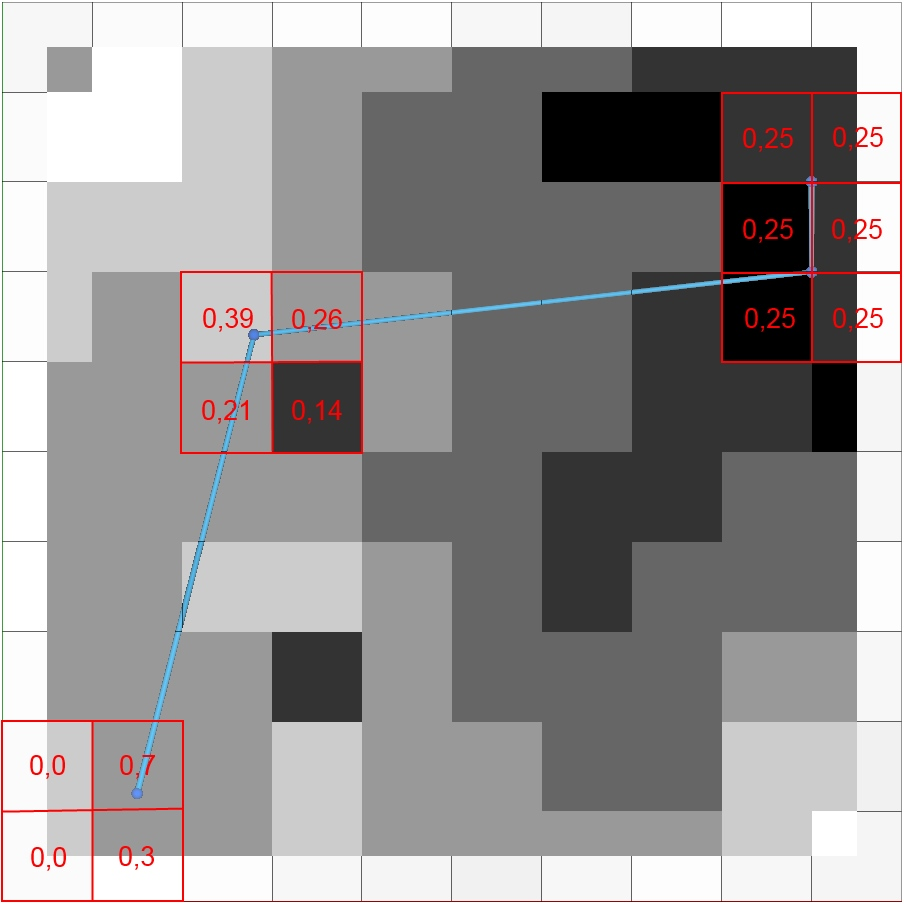
\includegraphics[width=.26\linewidth]{schema-dem}}\label{fig:schema:dem}}\,
  \subfloat[Mapping based on mesh]{\frame{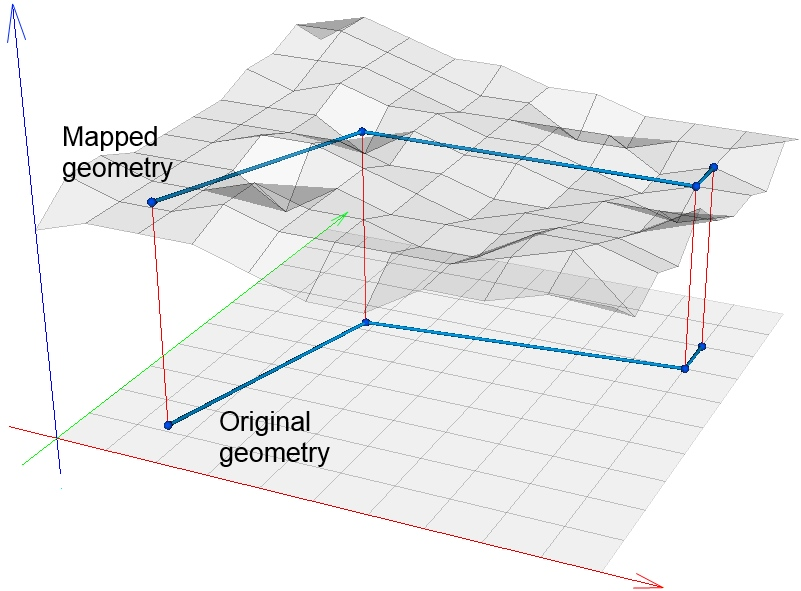
\includegraphics[width=.3525\linewidth]{schema-mesh1}}\label{fig:schema:mesh}}\,
  \subfloat[Additional geometric points]{\frame{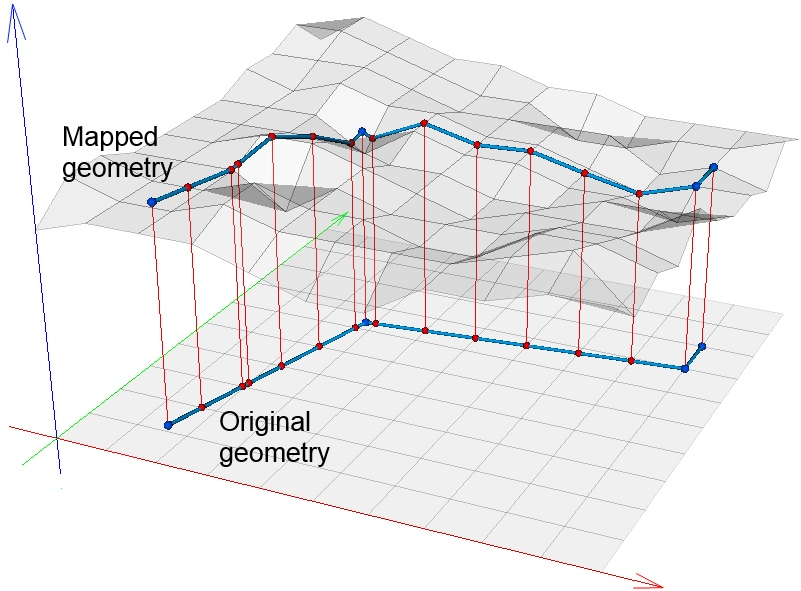
\includegraphics[width=.3525\linewidth]{schema-mesh2}}\label{fig:schema:points}}
  \caption{Schematic of mapping algorithms implemented in the \emph{OpenGeoSys Data Explorer}. \textbf{(a)}~Calculation of geometric point elevation based on weighted DEM pixels. \textbf{(b)}~Projection of points onto mesh surfaces via triangle line intersection. \textbf{(c)}~Inserting additional points into geometry at intersections of geometric lines with mesh element edges and nodes. Newly inserted points are marked in red.}
  \label{fig:geomappingschema}
\end{figure}

\subsection{Mapping Geometry}
\index{Mapping geometry}

Right-clicking a geometry in the Data View and selecting \cmd{Map geometry...} allows to add elevation information to all points of the selected geometry based on another data set (see fig. \ref{fig:dlgmods}a). This ``source''-data set can be either a mesh file or a file containing a digital elevation model (usually a *.asc or *.grd file). Both options can be selected from the pull down menu ``Map on data set''. In addition, this menu allows to select any mesh already loaded into \ogs to avoid loading the data set a second time. When selecting a DEM, geometric point will be given the elevation of the pixel they fall on when projected into the $(x,y)$-plane (see fig. \ref{fig:schema:dem}).

For a subsequent FEM-based simulation, it is usually better to map a geometric data set on the FEM mesh if the geometry will later be used for assigning boundary conditions. The mapping-dialogue offers two options for this case:

\begin{enumerate}
\item All geometric points $p_i \in P$ are mapped to the exact elevation of the mesh at the position of the point $p_i$ in the $(x,y)$-plane, i.e. to the point where a vertical line through $p_i$ intersects the mesh (see fig. \ref{fig:schema:mesh}).
\item In addition to the previous method, additional points are added whenever polylines projected onto the $(x,y)$-plane intersect mesh nodes or edges that have also been projected onto the $(x,y)$-plane (see \ref{fig:schema:points}).
\end{enumerate}

The second method will often result in larger geometry data sets, but also in a much better mapping. If unsure which method to use, it makes sense to try both and select the subjectively best result afterwards.


\section{Time Series and Stratigraphic Data to Observation Sites}
\index{Time series data}\index{Stratigraphic data}

For observation sites within the ``Stations'' Data View it is possible to display additional information such as logger data at the site or the stratigraphy at a borehole.

To view the additional information of an observation site load a stn-file into the programme and right-click on any observation site in the data view. You will see either the menu entry ``View Stratigraphy...'' for a borehole or ``View Diagram...'' for a station. While a borehole will always have strategraphic data (at least one layer over its whole length), not all stations will have time series data attached (this needs to be specified in the input file). If such data exists, a dialogue will open which allows to set a few parameters: A start and end date are set based on the data in the attached time series file for this station. This date can be changed to only display a subset of the data. There are also checkboxes for all all time series contained in the file which allow to specifically select only the time series the user wants to see. Upon pressing OK a new window will open, displaying the requested information.

\section{Generating and Modifying Meshes}

This section summarises the various way meshes can be created or modified using OpenGeoSys. Often functionality will be limited to a certain type of meshes, i.e. 2D meshes or 3D meshes. Usually the mesh dimension is based on the dimension of the elements within that mesh. For example, a triangle-mesh is 2D, a tetrahedra-mesh is 3D. For mixed element meshes, we find the maximum dimension of all the elements contained in that mesh to determine the mesh dimension. For example, a mesh containing tetrahedra (3D) and triangles (2D) is a 3D mesh; a mesh containing quads (2D) and lines (1D) is a 2D mesh; etc.

\subsection{Creating Meshes from Geometry}
\label{meshcreation}\index{Creating meshes}

By selecting \cmd{Tools\ra Mesh Generation...} a dialogue that allows the user to create meshes using information currently present in the programme. For this to work, the open-source mesh generating software GMSH\footnote{http://geuz.org/gmsh/} needs to be installed and be available from the location of the Data Explorer (i.e. located in the same directory or findable, e.g. via PATH-variable under MS Windows).

The user can select any geometry and observation sites that should be considered for generating the mesh. It is necessary that at least on polyline in any of the selected geometries is closed (i.e. is a polygon) and will serve as an outer boundary to the resulting mesh. Any further polygons found in the geometry will be meshed, polygons within polygons will simply be integrated within the encompassing larger shape. Note that all points of every data set considered for mesh generation and located within the outer boundary will be included as nodes in the final mesh. Therefore it makes sense to check if consecutive points of polylines are unnecessarily close together or too far apart.

Upon pressing \cmd{OK} a geometry-file (*.geo) for GMSH is written, GMSH is called to create the mesh and the newly created mesh is at once imported in the \ogs-Data Explorer. If not specified otherwise, the geo-file will be deleted again after the mesh has been created.

There is an \cmd{Advanced}-Tab in this dialogue that allows to set a number of parameters for the mesh. Most importantly, it can be chosen, if the new mesh should be adaptive or homogeneous. An adaptive mesh{Adaptive Meshes} is refined towards points or lines specified in the geometry while a homogeneous mesh has elements of roughly the same size everywhere in the domain (see figure \ref{fig:meshing}).

\begin{figure}[tb]
\begin{center}
\subfloat[Geometry]{\includegraphics[width=0.3\linewidth]{meshing-geo}\label{meshing-geo}}\enspace
\subfloat[Homogeneous mesh]{\includegraphics[width=0.3\linewidth]{meshing-hmg}\label{meshing-hmg}}\enspace
\subfloat[Adaptive mesh]{\includegraphics[width=0.3\linewidth]{meshing-adp}\label{meshing-adp}}
\end{center}
\caption{Meshing using geometric data and observation sites.} \label{fig:meshing}
\end{figure}

The specific parameters for adaptive meshes are:
\index{Adaptive meshes}
\begin{itemize}
\item \textbf{Max. number of points in Quadtree leaf:} Generally speaking, the smaller this number the more refined the resulting mesh will be. \\
    To give a more detailed explanation, basic knowledge about \emph{quad tree} data structures \footnote{http://en.wikipedia.org/wiki/Quadtree} is necessary: A tree structure is constructed by a sequential subdivision of the domain based on the distribution of relevant points in space. The criterium if a segment compromising a leaf is further refined is dependent on the number of points located within that segment. The size of the parameter relates to the maximum allowed size of mesh elements and additional points (\emph{Steiner points}) will be added to the data set to ensure the a certain refinement is guaranteed anywhere within the domain. Therefore, larger numbers of that parameters will usually result in coarser meshes while smaller numbers will result in finer meshes. \emph{Note that this is technically not a correct explanation as results are heavily dependent on how many points are located in certain sub-divisions of the domain, the existence of point clusters, etc.} See figure \ref{fig:quadtree} for an example.
\item \textbf{Mesh density scaling for points:} This is a scaling factor for the above parameter allowing for a refinement towards points located within the outer boundary. Again, smaller values will result in finer meshes.
\item \textbf{Mesh density scaling for stations:} This is exactly the same kind of scaling factor as for the option above, only for refinement towards observation sites, allowing a different mesh density for different regions of the mesh.
\end{itemize}

\begin{figure}[tb]
\begin{center}
\includegraphics[width=0.95\linewidth]{quadtree}\label{quadtree}
\end{center}
\caption{Adaptive meshing of geometry. The left column depicts polyline and points that need to be meshed. In the middle the resulting quad trees can be seen, the upper on generated with a maximum of two points per leaf, the lower one with 10 points per leaf. The resulting meshes are shown on the right side. Notice that regions where no information is available have roughly the same element size while elements where point information is given differ vastly in element size.} \label{fig:quadtree}
\end{figure}

Likewise, you can select an \textbf{element size}\index{Element size} for homogeneous meshes.\index{Homogeneous meshes} Here, too, a smaller number will result in a finer mesh, as the value specifies the maximum edge length of mesh elements.

\bigskip

Default parameters for all options are already predefined and have worked well with most examples that have been tested. However, results are heavily dependent an the bounding box of all data sets used for mesh generation. Often it is necessary to play around with these numbers a bit. Usually it makes sense to start with larger parameters that result in coarser meshes to get a rough idea what the final mesh will look like and where potential problems may be located.

\subsection{Creating Meshes from Raster Files}
\label{meshraster}\index{Creating meshes}

\begin{figure}[tb]
\begin{center}
\subfloat[Raster]{\includegraphics[width=0.3\linewidth]{rastermesh1}\label{rastermesh1}}\enspace
\subfloat[Elevation]{\includegraphics[width=0.3\linewidth]{rastermesh2}\label{rastermesh2}}\enspace
\subfloat[Materials]{\includegraphics[width=0.3\linewidth]{rastermesh3}\label{rastermesh3}}
\end{center}
\caption{Creating meshes from raster files: Pixels can be either represented as a set of two triangles (Fig. \ref{rastermesh2}) or a square (Fig. \ref{rastermesh3}), intensities may represent elevation (Fig. \ref{rastermesh2}) or materials (Fig. \ref{rastermesh3}).}
\label{fig:rastermesh}
\end{figure}

A completely different way to create a mesh is based on image or raster files, such as *.asc-files from ArcGIS. If the file is loading into the Data Explorer it will appear in the Visualisation Pipeline only. Right clicking the pipeline item allows to select the menu item \cmd{Convert Image to Mesh...}. A dialogue allows the parameterise how exactly this conversion should be performed. Specifically, it is possible to select a mesh element type for representation of pixels and a way in which grey-values should be interpreted\footnote{Meshes can also be generated from colour images. However, the colours will be converted to grey-values via $g = 0.3*\text{red}+0.6*\text{green}+0.1*\text{blue}$.}.

For the first parameter, pixels can be converted into a square (i.e. a quadrilateral element) or two rectilinear triangles (i.e. two triangle elements). In the future it is also planned to offer cubes (i.e. a hexahedron) for multi-layered images.

For the second parameter the user can decide wether pixel values should be interpreted as elevation (which is useful if the raster represents a digital elevation model) or if the grey-values should be assigned as scalar values to the mesh elements. As a third alternative, these values can also be completely ignored (see Fig. \ref{fig:rastermesh} for examples).

If the raster file contains ``NoData''-values (this is common in raster files created with a Geographic Information Systems such as ArcGIS), these values are ignored and will not appear as mesh-elements after the conversion  (i.e. despite the raster file always being rectilinear the resulting mesh may have an arbitrary boundary defined be pixels actually containing information).

\subsection{Converting Meshes to Geometry}
\index{Convert Mesh to geometry}
\index{Mesh to geometry conversion}

A 2D mesh loaded into \ogs can be converted into a geometry data set by right-clicking the mesh and selecting \cmd{Convert to geometry}. This will copy mesh nodes to geometric points and the mesh itself to a triangulated surface. In the same way, a 2D mesh can be converted into an ESRI shape file (by selecting \cmd{Export to Shapefile...}). The resulting file will be of type SHPT\textunderscore POLYGON and each mesh element will be represented as a polygon within the shape file.

\subsection{Extracting the surface of a mesh}

It is possible to extract the surface of a 3D mesh by right-clicking the mesh and selecting \cmd{Extract surface}. This will result in a 2D mesh of the surface elements of the 3D mesh, i.e. all elements visible when viewing the mesh from $z+$ direction.

Topologically, the result will consisting of all faces of 3D mesh elements where the surface normal n satisfies $|n - \left[0, 0, 1\right]|<90\degree$. Note that for certain meshes the result might also contain elements not actually connected to the surface if these unconnected elements also satisfy the constraint given above (e.g. if the 3D mesh contained holes).


\subsection{Mapping of Meshes based on DEMs}
\label{meshondemmapping}
\index{Mapping meshes}
\index{Adding mesh layers based on DEM}

For mapping a 2D mesh based on a DEM or for adding multiple layers based on elevation profiles, right-click the mesh and select \cmd{Edit mesh...}. The dialogue will require the number of layers to be mapped for this mesh. A ``layer'' in the sense of the underlying simulation algorithms, consists of 3D elements. Therefore a 2D mesh technically consists of $0$ layers. Subsequently, when mapping a 2D mesh, it is necessary to specify the number of layers as $0$ and use one DEM to actually map the layer. Likewise, one layer will require (at least) two digital elevation models (DEM) to be specified, one for the top-face of the elements and one for the bottom-face.

In general, $n+1$ raster files in *.asc format are required for mapping $n$ mesh layers. The dialogue also allows to select one additional DEM-file called ``Surface''. If a 2D mesh should be mapped, this is the only file that needs to be specified. For a 3D mesh it is optional and serves a different purpose: The raster files given for the mapping usually represent the boundaries between subsurface layers (e.g. Statigraphic layers, aquifers, etc.). These are often interpolated from borehole information (e.g. using the kriging algorithm). This may result in an upper boundary of the subsurface model that is located above the actual surface of the model region. For multi-layered meshes the mapping will first be performed on all subsurface layers and the resulting mesh will then be intersected with the optional Surface DEM (i.e. the digital terrain model), thus effectively cutting away all elements located above surface. \emph{Note that currently the check if two layers are intersecting each other does \emph{not} work correctly for any other layers except the DEM!}

\begin{figure}[tb]
\begin{center}
\subfloat[Surface Mesh]{\includegraphics[width=0.3\linewidth]{AmmerSurface}\label{fig:AmmerSurface}}\enspace
\subfloat[Fixed thickness]{\includegraphics[width=0.3\linewidth]{AmmerSubsurface}\label{fig:AmmerSubsurface}}\enspace
\subfloat[Based on DEM]{\includegraphics[width=0.3\linewidth]{AmmerFinal}\label{fig:AmmerFinal}}
\end{center}
\caption{Mapping meshes based on raster files: \textbf{(a)} original surface mesh, \textbf{(b)} adding subsurface layers of fixed size, \textbf{(c)} adding subsurface layers based on elevation models. In a final step the subsurface model is intersected with the terrain model (i.e. the actual surface elevation).}
\label{fig:RasterMapping}
\end{figure}

For meshes containing only 2D elements there is also an option ``Remove mesh nodes at NoData values''. Per default this option is switched off as the correctness of the result is depending on the element size in these NoData locations.

\subsection{Adding Layers of Fixed Size}
\label{fixedsizelayers}
\index{Adding mesh layers of fixed size}

Besides adding subsurface layers using DEM-profiles as described in the previous section, a 2D mesh can also be extruded into a 3D mesh by copying the 2D mesh layer a specified number of times and then connected any two neighbouring layers by creating 3D elements from all corresponding 2D elements (i.e. two triangles are connected and form one prism-elements, two quadrilateral elements form one hexahedron). This functionality can also be accessed by right-clicking on a 2D mesh in the data view and selecting \cmd{Edit Mesh...}. Again, specify the number of layers you would like to add and select \cmd{Add layers with static thickness}. After that the thickness of each layer needs to be specified.

\subsection{Analyse Mesh Quality}
\index{Mesh quality}

You can visualise the quality of a given mesh by right-clicking on the mesh in the respective Data View and selecting \cmd{Check Mesh Quality...}. This currently allows to choose between four implemented measurements for mesh element quality. The result of choosing any of these modes is a colour-codes overlay of the mesh where every element is assigned a quality in $[0,1]$. You can select this overlay in the visualisation pipeline and specify thresholds to select a certain range of quality and see which element fall into that range. \emph{(Note: You might need to manually set the correct scalar array for visualising mesh quality. The appropriate data can be chosen by selecting in ``C-Selection'' in the \cmd{Active Scalar} pull-down menu.}

\begin{figure}[tb]
\begin{center}
\subfloat[Edge Aspect Ratio]{\includegraphics[width=0.3\linewidth]{MshQualEdgeRatio}\label{fig:mshqual1}}\enspace
\subfloat[Element Area]{\includegraphics[width=0.3\linewidth]{MshQualArea}\label{fig:mshqual2}}\enspace
\subfloat[EquiAngle Skewness]{\includegraphics[width=0.3\linewidth]{MshQualEquiAngle}\label{fig:mshqual3}}
\end{center}
\caption{Examples for colour coded mesh quality measurements.} \label{fig:mshqual}
\end{figure}

The currently implemented measures are the following:
\begin{itemize}
\item \textbf{Aspect Ratio of Edge Length:} Analyses the ratio of shortest to longest edge of every element. Equilateral elements are often considered superior and better suited for FEM simulation, therefore these elements are rated ``1'' with their quality degrading with increasing differences in edge length. Each element is assigned the value of the highest ratio between any two of its edges. This is a good measure for triangle elements but might be not as good as others. See figure \ref{fig:mshqual1}.
\item \textbf{Area of 2D Elements:} Compares the area of all 2D elements (this includes the faces of 3D elements!) by assigned ``1'' to the element with the largest area and ``0'' to the element with the smallest area. See figure \ref{fig:mshqual2}.
\item \textbf{Volume of 3D Elements:} As with the area-criterion, this measure compares the volume of 3D mesh elements. 2D elements are ignored when this option is selected.
\item \textbf{Angles between Adjacent Edges:} Calculates the maximum deviation of an angle between any two adjacent edges of the element from the ``optimum'' angle, i.e. the angle of an equiangular element. This optimum angle is $90\degree$ for triangles or tetrahedra and $90\degree$ for quadrilateral or hexahedral elements. This measurement is called \emph{EquiAngle Skewness} and given by
    \begin{equation}
    s = \max\left[\frac{\theta_{max}-\theta_{opt}}{180-\theta_{opt}},\frac{\theta_{opt}-\theta_{min}}{\theta_{opt}}\right]
    \end{equation}
    where $\theta_{max}$ is the maximum angle between any two edges found in the element, $\theta_{min}$ is the minimum angle and $\theta_{opt}$ is the optimum angle.
    See figure \ref{fig:mshqual3}.
\end{itemize}

The quality measure best suited for a given mesh might depend on the process you want to simulate using this mesh. For instance, processes such as groundwater recharge consist mainly of layered flows, meaning that large differences between horizontal and vertical element surfaces might have no effect on a correct result. The simulation of mass transport processes explicitly requires a fine mesh resolution in vertical direction to ensure a stable solution.

\begin{figure}[tb]
\begin{center}
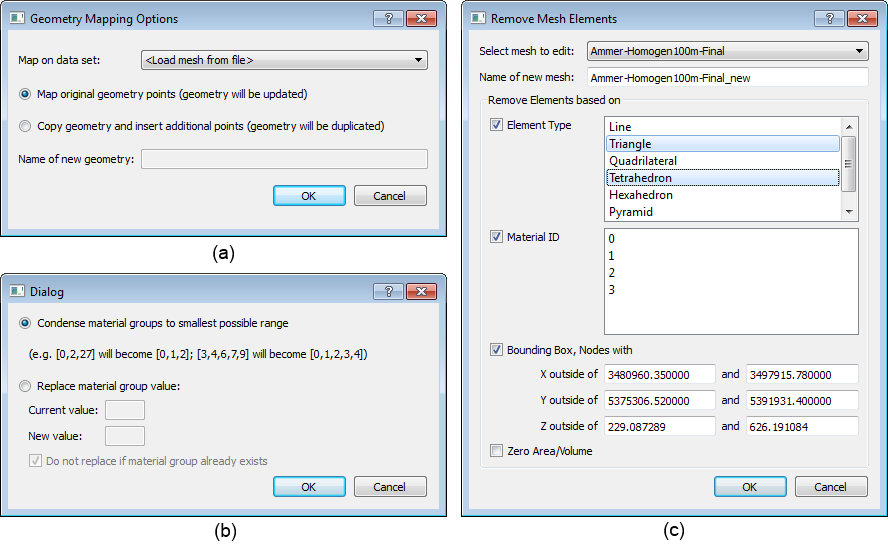
\includegraphics[width=0.8\linewidth]{dlg_mods}
\end{center}
\caption{\ogs Data Explorer dialogs for modification of data sets: \textbf{(a)} Mapping geometry based on a mesh or DEM, \textbf{(b)} Changing the material groups of a mesh, \textbf{(c)} Remove elements from a mesh based on certain criteria.} \label{fig:dlgmods}
\end{figure}

\subsection{Changing Material Groups}
\index{Changing material groups}

Each element in a mesh is assigned a non-negative integer that specifies a material group this element belongs to. These material groups can be arbitrarily assigned. For instance, a mesh containing only two groups could name these groups ``17'' and ``98'' or use some different, arbitrary IDs. By right-clicking on a mesh and selecting \cmd{Edit Material Groups...} it is possible the change the ID of one or more groups or to merge groups (see fig. \ref{fig:dlgmods}b).

The two basic options are ``Condense material groups to smallest possible range'' and ``Replace material group value''. The first option will rename all material groups such that the group with the smallest ID will be assigned $0$, the group with the second-smallest ID will be assigned $1$, and so on. In a mesh with $10$ different material groups the largest existing ID will be $9$ after processing the mesh.

The second option allows to specifically rename the ID of any group from the current value $A$ to any new value $B$. If $B$ already exists, the programme will give a warning and ask the user if the renaming process should really be started, thus merging groups $A$ and $B$.

\subsection{Removing Duplicate or Unused Mesh Nodes}
\index{Removing mesh nodes}

As with loading geometric data, certain checks are performed when loading meshes. The programme will automatically removed mesh nodes that are not part of any mesh element. Also, it is possible to remove duplicate mesh nodes, i.e. nodes that are located at the exact or almost exact same position as other nodes. The results for meshes are a bit more complicated as for geometries and this might require a restructuring or subdivision of mesh elements (i.e. if one node is removed from a prism-element, restructuring will result in two tetrahedra).

\subsection{Removing Mesh Elements}
\index{Removing mesh elements}

\ogs allows to remove mesh elements based on a number of criteria. A dialogue for selecting which elements to remove can by opened by selecting \cmd{Tools \ra Remove Mesh Elements...} (see fig. \ref{fig:dlgmods}c). It is necessary to specify the mesh from which elements need to be removed as well as the name of the resulting new mesh. Possible options based on which elements may be removed include element type, material group, bounding box as well as zero volume elements. The dialogue allows to select any combination of these constraints. An error message will be given if the selected criteria would result in removing either none or all of the elements in the selected mesh.



\section{Modelling Data}

\subsection{Creating Processes}
\index{Creating processes}

It is possible to add processes to the workflow in the Modelling-tab by pressing the \cmd{Add process...}-button. A dialogue will open that allows to select a process type and an associated primary variable. As of version 5.2.07 this has no effect on output files except for boundary conditions being grouped under these processes and being removed upon removing the process (via right-click \cmd{Remove process}).

\subsection{Creating FEM Conditions}
\index{Creating FEM conditions}
\index{Creating boundary conditions}

It is possible to create FEM conditions based on geometric objects. By right-clicking on the respective point, polyline or surface and selecting \cmd{Set as FEM condition...} a setup dialogue will open (Fig. \ref{fig:CondSetupDlg}). Here, it can be specified for which process and primary variable the condition should be used and if it should be a boundary condition, a source term or an initial condition. Based on the geometrical object type and the selection of the condition type a number of distribution types will be available. For example, points as boundary conditions can only have \emph{Constant (Dirichlet)} distribution; lines as source terms can have \emph{Constant (Neumann)} or \emph{Linear (Neumann)} distribution, etc.

\begin{figure}[tb]
\begin{center}
\subfloat[FEM Condition Setup]{\includegraphics[height=4.0cm]{dlg_cond_setup}\label{fig:CondSetupDlg}}\enspace
\subfloat[Linear]{\includegraphics[height=4.0cm]{dlg_lin_dist}\label{fig:LinearDlg}}\enspace
\subfloat[Direct]{\includegraphics[height=4.0cm]{dlg_direct_dist}\label{fig:DirectDlg}}
\end{center}
\caption{Dialogues for creating of FEM Conditions.} \label{fig:CondSetup}
\end{figure}

While the assignment of values is easy for \emph{constant} distributions, it an get quite complex for \emph{linear} or \emph{direct} distributions. The FEM Condition Setup Dialogue will therefore contain a button ``Calculate Values'' instead of a textfield. Upon pressing this button a (different) dialogue will open to configure the values. For \emph{linear} distributions a table is displayed where for each point of the line a value can be inserted (Fig. \ref{fig:LinearDlg}). Conditions are only actually set up between points with given values. As an alternative it is possible to automatically insert the elevation (z-Coordinate) for each point of the line. For \emph{direct} distributions the dialogue will require to specify a raster file from which values are read for direct assignment to mesh nodes (Fig. \ref{fig:DirectDlg}). The user can select between a 1:1 assignment or a surface integration based on the area of the mesh elements the respective node is part of. In this case it is also possible to specify a scaling value to compensate for data files with different units of measurement.

For polylines or surfaces it is also possible to assign the conditions not directly on the geometric objects but instead on all points compromising the object. For example, a polyline consisting of 50 points can be either assigned one boundary conditions with a linear distribution or 50 boundary conditions on the respective points, each of which has a constant value.

Once created, FEM conditions can be saved by right-clicking associated process in the ``Modelling'' tab and selecting \cmd{Save FEM conditions...}. The user can specify the file format (XML or ASCII) and the type of conditions that should be written (boundary conditions, initial conditions, source terms or all of them).

\subsection{Changing FEM Conditions}
\index{Changing FEM conditions}

Conditions loaded into the \ogs Data Explorer can be edited simply by right-clicking the respective geometric object in the ``Modelling'' tab and selecting \cmd{Edit condition}. This will once again open the FEM Condition Setup Dialogue that is also used for creating conditions. For existing conditions the appropriate values will already have been selected and can now be changed. Changes in the corresponding files will only be written once the user actively saves these files again via \cmd{Save FEM Conditions...}



\chapter{Visualisation}

\section{Visualisation Properties}
\index{Visualisation settings}

Some properties of the render window can be modified by selecting \cmd{Settings\ra} \cmd{Visualisation Settings...}. The dialogue that opens allows you to change several global properties of the render window.

For any rendered scene in computer graphics a light source\index{Light} has to be specified. This is basically the equivalent to the sun or a lamp in the room.
\begin{wrapfigure}{r}{0.4\textwidth}
   \vspace{-15px}
   \begin{center}
     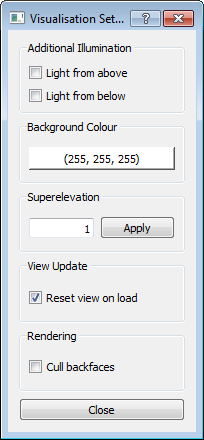
\includegraphics[width=0.36\textwidth]{dlg_vis_settings}
   \end{center}
   \vspace{-20px}
\end{wrapfigure}
The default setting in \ogs and many other tools is a light source identical with the camera, i.e. the light source always illuminates the part of an object in the render window that can be seen by the user. In some cases this illumination is not enough, though, and interesting parts of a rendered object may be covered by shadows. Therefore it is possible to switch on additional light sources above and below the object to ensure a full illumination of the scene.

The background colour\index{Background colour} of the render window can be changed to any arbitrary colour by clicking on the button displaying the current background colour. The button also displays the RGB-value of the currently selected colour.

A global superelevation\index{Superelevation} factor can be applied to all root objects in the visualisation pipeline. This overwrites all previously set superelevation factors and is especially useful when dealing with a large number of files, all of which should be assigned the same superelevation (e.g. when using \ogs projects, see section \ref{nativefileformats}).

Per default upon loading a new data set the 3D view is adapted to show the entire scene from above (i.e. the \emph{z+}-axis). This can be switched of by unchecking the ``Reset view on load'' option. This might be useful when making a series of screenshots with the exact same point of view.

Finally, it is possible to switch on backface culling\index{Backface culling}. This will result in rendering only triangles with normals directed towards the camera/observer. This improves rendering speed and may be useful for finding false ordered primitives.

\section{General Visualisation Options}
\label{genvisoptions}

For each graphics-object in the visualisation pipeline there a number of parameters that can be changed to make the object more easily distinguishable or to convey information contained in the data. These general options can be found in the \emph{Visualization Pipeline}-tab and are called ``Actor Properties'' (based on their use within VTK).

\begin{figure}[tb]
\begin{center}
\subfloat[Solid Color]{\includegraphics[width=0.3\linewidth]{colour-solid}\label{colour-solid}} \enspace
\subfloat[Default colour table]{\includegraphics[width=0.3\linewidth]{colour-default}\label{colour-default}}\enspace
\subfloat[User-defined colours]{\includegraphics[width=0.3\linewidth]{colour-user}\label{colour-user}}
\end{center}
\caption{Each object is assigned a random solid colour as well as a default colour table based on a temperature scale (from blue to red). The solid colour can be adjusted via the ``Diffuse Color''-option (see section \ref{genvisoptions}), the colour table can be adjusted by loading a user-defined *.xml file via the ``Add color table...''-option (see section \ref{specvisoptions}).} \label{fig:colours}
\end{figure}

Specifically these parameters are:

\begin{itemize}
\item \textbf{Diffuse Color:}\index{Changing Colour} Each item is assigned a colour which is used for rendering the object in 3D space. This colour can be changed here (see figure \ref{colour-solid}). If the item is assigned one or more scalar arrays (see next item) then this colour is displayed upon selecting \emph{Solid Color}.
\item \textbf{Active Scalar:}\index{Changing scalar values} Each visualisation object has an assigned colour called \emph{Solid Color} which is used in the rendering process (see above). However, some data sets contain additional information, such as individual values assigned to each point or mesh node as well as to any triangle or mesh element. Examples are material groups for meshes, the concentration of chemical substances, values assigned as boundary conditions, etc. Such information is called a \emph{Scalar Array} assigned to the data set and can be selected here. This additional data is then employed in the rendering of object (see figure \ref{colour-default}). In theory, an object can have any number of such scalar arrays. However, only one of these can be selected at any time.\\
    On the right side of the `Active Scalar'-pulldown-menu is also a button for re-adjusting the colour table. This might be necessary to use after parameter changes for certain filters, when the colour lookup table for this specific array is not automatically adjusted.
\item \textbf{Visible Edges:}\index{Edges} Some objects (such as meshes) are composed of a combination of lines (edges) and surfaces. While the colour of the surfaces can be set using the \emph{Diffuse Color}-button, the colour of the edges can be changed here. Furthermore the rendering of edges can be switched off entirely by unchecking the box next this option.
\item \textbf{Opacity:}\index{Opacity}\index{Transparency} This determines if an object appears to be completely or partially transparent or not. A value of $0$ (leftmost position of the slider) makes the object completely transparent, a value of $1$ (rightmost position) makes the object completely opaque.
\item \textbf{Scaling Factor:}\index{Scaling} Super-elevates the data by the given factor. Values $x>1$ will emphasise differences in height while values $0<x<1$ will compress the extent in $z$-direction.
\item \textbf{Translation:}\index{Translation} Any data set can be moved in x, y or z-dimension so data sets can be set in relation to each other for comparison or layered visualisation.
\end{itemize}


\section{Modification and Export Options}
\label{specvisoptions}

When right-clicking an object in the \emph{Visualisation Pipeline}, a number of options appear for modifying, converting or exporting that specific object. Not all options listed here apply to all types of pipeline items.

\begin{itemize}
\item \textbf{Add filter...:} Allows to apply a filter to the current object. There are many options and possibilities here and \ogs will add more filter-options over time. For details on that option see section \ref{filters}.
\item \textbf{Add color table...:}\index{Colour lookup tables} Allows the assignment of a specific colour table to the currently selected scalar array (see figure \ref{colour-user}). The colour table is loaded from a *.xml-file and has the same format as ParaView\footnote{ParaView is an open-source data analysis and visualisation application for VTK data. It can be downloaded at \url{http://www.paraview.org/}}-colour-lookup-tables.\index{ParaView}
    New lookup tables and can therefore be created or edited using ParaView and all colour tables used in \ogs can conversely be imported into ParaView.
    The option to change colour tables is available for all objects, although for image data it is not available via right-click but needs to be called as a filter (see section \ref{filters}).
\item \textbf{Convert to Mesh...:} Allows to convert an object of the VTK-data type ``Unstructured Grid'' to be converted into an \ogs mesh. Objects of that type are basically meshes that are stored in a different data structure than ``normal'' \ogs meshes. Therefore, this specifically allows the conversion of imported VTK-files to \ogs meshes. Upon conversion the converted mesh will also appear in the respective \emph{Data View.}\\
    This option is available for all objects of type ``VTK\_UN\-STRUCT\-URED\_GRID'' (i.e. all mesh objects).
\item \textbf{Convert Image to Mesh...:} Generates an \ogs mesh based on a given raster file (see figure \ref{Filter-Img4}). For more information, see section \ref{meshraster}. This options is only available for image data (i.e. raster files).
\item \textbf{Export to VTK:}\index{VTK export} All objects displayed the render window are technically VTK-objects. Choosing this option saves these objects in VTK-format to a file. They can then be used in any software supporting this format (e.g. Paraview).
\item \textbf{Export to OpenSG:}\index{OpenSG export} Converts objects into OpenSG format (*.osg). This is another open source graphics format. It is also the format used by the UFZ VisLab. Specifically, this also implies that \emph{anything} that can be visualised in \ogs can also be exported to OpenSG and be presented in the VisLab. This option only appears if an OpenSG-library is linked from \ogs.
\item \textbf{Export to FBX:}\index{FBX export}\index{Autodesk export}\index{Unity export} Converts objects into Autodesk format (*.fbx). This is yet another graphics format, originally used by AutoDesk but also supported by other graphics software such as Unity3D. This option only appears if an FBX-library is linked from \ogs.
\end{itemize}

\section{Applying Filters for Visualisation}
\label{filters}

In contrast to the options detailed in the previous section, filters are modifications of the actual graphics object to enhance, reduce or deform certain aspects of these objects.\footnote{One might argue that this definition also holds true for the assignment of specific color tables which is accessed via right-click on an object. This inconsistency originates in the data structures the objects are stored in and in defining an easy-to-use workflow for using this functionality.}.

Filters can be applied by right-clicking on an object in the visualisation pipeline and selecting \cmd{Add filter...}.\index{Adding filters}\index{Filter} A dialogue will open where a number of available filters can be selected. As with other visualisation functionality described before, filters will only be displayed for objects they can be applied to. However, this does not mean that the result of any filter will make sense for any object where it can be applied. Also note, that it is possible (and sometimes useful) to apply filters to filters to extract certain information bit by bit.
%
\begin{figure}[tb]
\begin{center}
\subfloat[Raster data]{\includegraphics[width=0.4\linewidth]{Filter-Img1}\label{Filter-Img1}}\enspace
\subfloat[Apply lookup table to image]{\includegraphics[width=0.4\linewidth]{Filter-Img2}\label{Filter-Img2}} \\
\subfloat[Image to bar chart]{\includegraphics[width=0.4\linewidth]{Filter-Img3}\label{Filter-Img3}}\enspace
\subfloat[Convert Image to Mesh]{\includegraphics[width=0.4\linewidth]{Filter-Img4}\label{Filter-Img4}}
\end{center}
\caption{\ogs functionality applicable to image-/raster-data.} \label{fig:filter:raster}
\end{figure}
%
A short description for all available filters is given in the following:

\subsubsection{Apply lookup table to image}
\bstart{Applicable to:} Image Data
\index{Colour lookup tables}

\bstart{Effect:} Applies a color table to images. The color table can be read from a *.xml-file. If no file is specified, a default color table is automatically generated, replacing grey values with a temperature scale (i.e. dark colours are blue, light colours are red). In the resulting image, certain gradients might be better discernable or certain values might be highlighted. See figure \ref{Filter-Img2}.

\bstart{Remarks:} \emph{This is similar to applying a pre-defined colour table to a geometry- or mesh object. The implementation as a filter for images is based on the very different structure of image objects in the graphics library VTK which is used for visualisation.}

\begin{figure}[tb]
\begin{center}
\subfloat[Geometry Data]{\includegraphics[width=0.4\linewidth]{Filter-Poly1}\label{Filter-Poly1}}\enspace
\subfloat[Points to Spheres]{\includegraphics[width=0.4\linewidth]{Filter-Poly2}\label{Filter-Poly2}} \\
\subfloat[Lines to tubes]{\includegraphics[width=0.4\linewidth]{Filter-Poly3}\label{Filter-Poly3}}\enspace
\subfloat[Extract cells by threshold]{\includegraphics[width=0.4\linewidth]{Filter-Poly4}\label{Filter-Poly4}}
\end{center}
\caption{\ogs functionality applicable to geometry data. In figure \ref{Filter-Poly2} ground water stations in the area have been emphasised. In figure \ref{Filter-Poly4} a threshold filter has been applied to the tube-filtered data from figure \ref{Filter-Poly3} to select only the river network of the depicted area from the geometric data.} \label{fig:filter:poly}
\end{figure}

\subsubsection{Apply texture to surface}
\index{Textures}\index{Raster files}\index{Raster files}\index{NetCDF files}
\bstart{Applicable to:} Surfaces, Meshes

\bstart{Effect:} Allows to map an image/raster on a surface or mesh. This might make sense for adding more information to a given object such as land use classes, precipitation, etc. Possible formats for loading textures include all supported raster formats as well as netCDF files (see \ref{Import File Formats}). An example is shown in figure \ref{Filter-Mesh4}.

\subsubsection{Elevation-based colouring}
\bstart{Applicable to:} Geometry, Meshes

\bstart{Effect: } Applies a colour to each point depending on the z-coordinate of that point, assuming that this denotes height in metres. The pre-defined colour scale starts with blue up to a height of $0$ metres (i.e. sea level), which is then slowly changing to green (150\,m) and yellow (450\,m) and then changing to red.. See figure \ref{Filter-Mesh2}.

\bstart{Remarks:} \emph{In theory these values can be changed. This is, however, currently not possible using the GUI. It is very easy in the source code, though, as this just constitues a predefined colour lookup table.}

\begin{figure}[tb]
\begin{center}
\subfloat[Multilayered Mesh]{\includegraphics[width=0.4\linewidth]{Filter-Mesh1}\label{Filter-Mesh1}}\enspace
\subfloat[Elevation-based colouring]{\includegraphics[width=0.4\linewidth]{Filter-Mesh2}\label{Filter-Mesh2}} \\
\subfloat[Extract cells by threshold]{\includegraphics[width=0.4\linewidth]{Filter-Mesh3}\label{Filter-Mesh3}}\enspace
\subfloat[Apply texture to surface]{\includegraphics[width=0.4\linewidth]{Filter-Mesh4}\label{Filter-Mesh4}}
\end{center}
\caption{\ogs functionality applicable to meshes.} \label{fig:filter:mesh}
\end{figure}

\subsubsection{Extract cells by threshold}
\index{Threshold filter}
\bstart{Applicable to:} Geometry, Observation Sites, Meshes

\bstart{Effect:} Geometric objects as well as mesh layers have unique IDs which allows to assign different colours to different objects. This filter furthermore allows to select a range of objects which should be displayed while all other objects are blanked out. This allows for the visualisation of one or more specified stratigraphic layer, polyline or mesh layer. See figures \ref{Filter-Poly4} and \ref{Filter-Mesh3}. The filter is always applied to the currently selected scalar array. For instance, given a mesh containing scalar arrays for material group and groundwater head, this filter may be used to select a range of materials (e.g. only materials with IDs 5--7) or regions with a certain groundwater head (e.g. $\text{head}>7.2\,m$).

\subsubsection{Generate contours based on scalar fields}
\index{Contour filter}
\bstart{Applicable to:} Meshes

\bstart{Effect:} Given a scalar field this filter will output contour lines of meshes containing 2D elements and contour surfaces for meshes containing 3D elements. The number of contours that should be displayed can be defined in the filter properties as well as the minimum and maximum value for the calculated contours. The chosen number of contours will that be calculated on the selected scalar field in equidistant intervals between the selected minimum and maximum value. The colours of the contours are automatically chosen based on these scalar values.

\subsubsection{Image to bar chart}
\bstart{Applicable to:} Image Data

\bstart{Effect:} Each pixel is assigned a bar depending on the grey value of the pixel. Also, the colour changes of that bar changes according to its height. See figure \ref{Filter-Img3}.

\bstart{Remarks:} \emph{This filter takes a lot of time for large images as the result becomes very complex from a computer graphics point of view. The intention is to use it for low resolution raster data of phenomena such as precipitation, etc.}

\emph{This is also a good example on the combination of the successive application of these filters. This one combines `Image to vertical lines', `Lines to tubes' and `Elevation-based colouring'.}

\subsubsection{Image to vertical lines}
\bstart{Applicable to:} Image Data

\bstart{Effect:} Plots vertical lines for every pixel of a raster with each line having a height depending on the raster's grey value.

\bstart{Remarks:} \emph{This is a filter that is needed for the correct application of other filters. It is probably not of much use by itself.}

\subsubsection{Lines to tubes}
\index{Tube filter}
\bstart{Applicable to:} Geometry, Observation sites

\bstart{Effect:} A geometric line has independent of the current zoom level always a thickness of $1$. This filter allows to assign a `real' thickness to line-objects that also changes according to the current zoom. See figure \ref{Filter-Poly3}.

\subsubsection{Points to spheres}
\index{Sphere filter}\index{Glyph Filter}
\bstart{Applicable to:} Geometry, Observation sites

\bstart{Effect:} A geometric point has independent of the current zoom level always a diameter of $1$. This filter allows to assign a `real' radius to point-objects that also changes according to the current zoom. See figure \ref{Filter-Poly2}.

\subsubsection{Surface filter}
\index{Surface filter}
\bstart{Applicable to:} Meshes

\bstart{Effect:} Extracts the outer surface of a mesh.

\bstart{Remarks:} \emph{This is a filter that is needed for the correct application of other filters. It is probably not of much use by itself.}


%\chapter{Example Workflows}
\index{Workflows}

\section{Creating a Hydrogeological Subsurface Mesh}
\label{sec:dataexplorer:workflow}

\begin{figure}[!h]
\begin{center}
\subfloat[Surface model data]{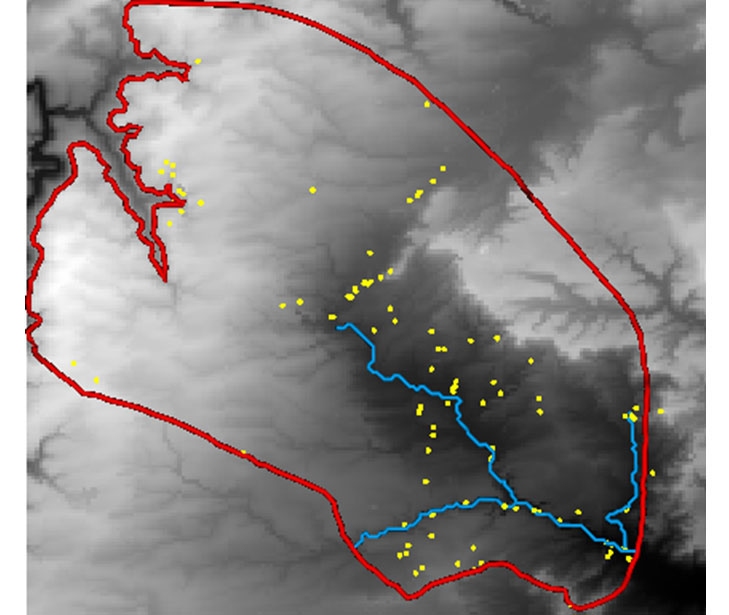
\includegraphics[width=0.48\linewidth]{ammer_gis.png}\label{fig:kr:ammer_gis}}\enspace
\subfloat[Surface model data]{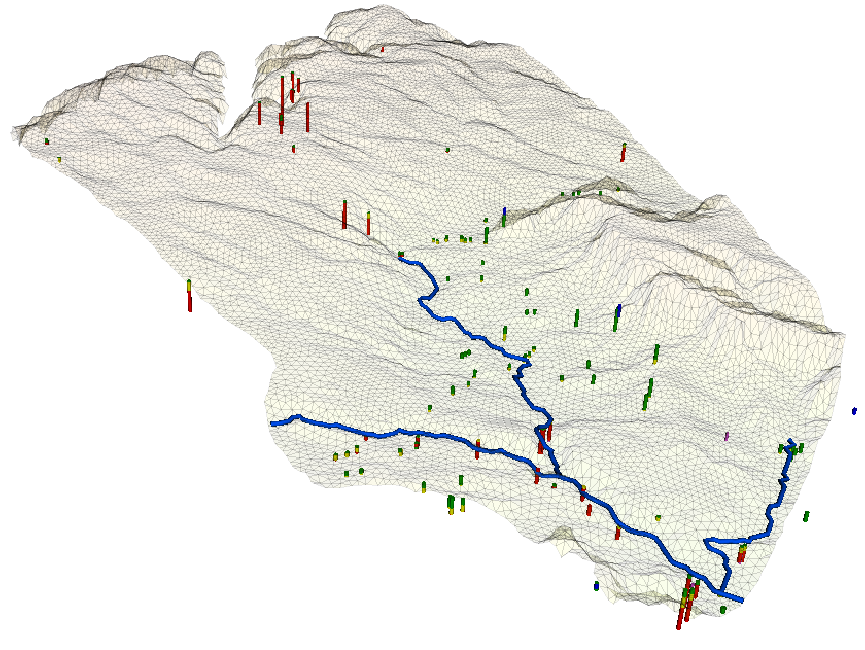
\includegraphics[width=0.48\linewidth]{ammer_sfc.png}\label{fig:kr:ammer_2d}}\\
\subfloat[Subsurface model]{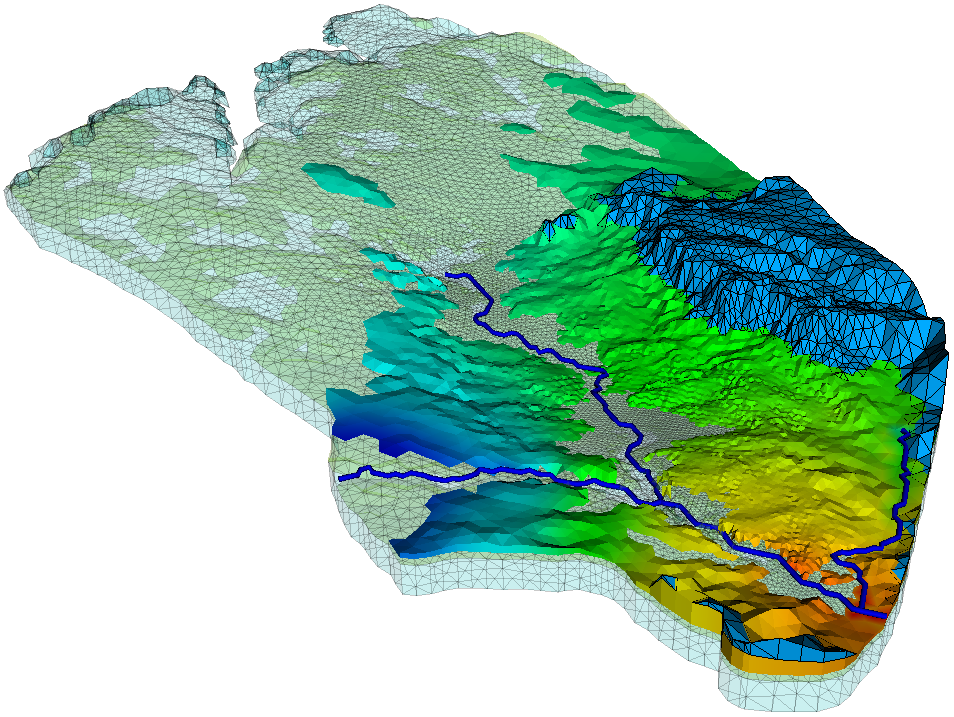
\includegraphics[width=0.48\linewidth]{ammer_3d.png}\label{fig:kr:ammer_3d}}\enspace
\subfloat[Simulation results]{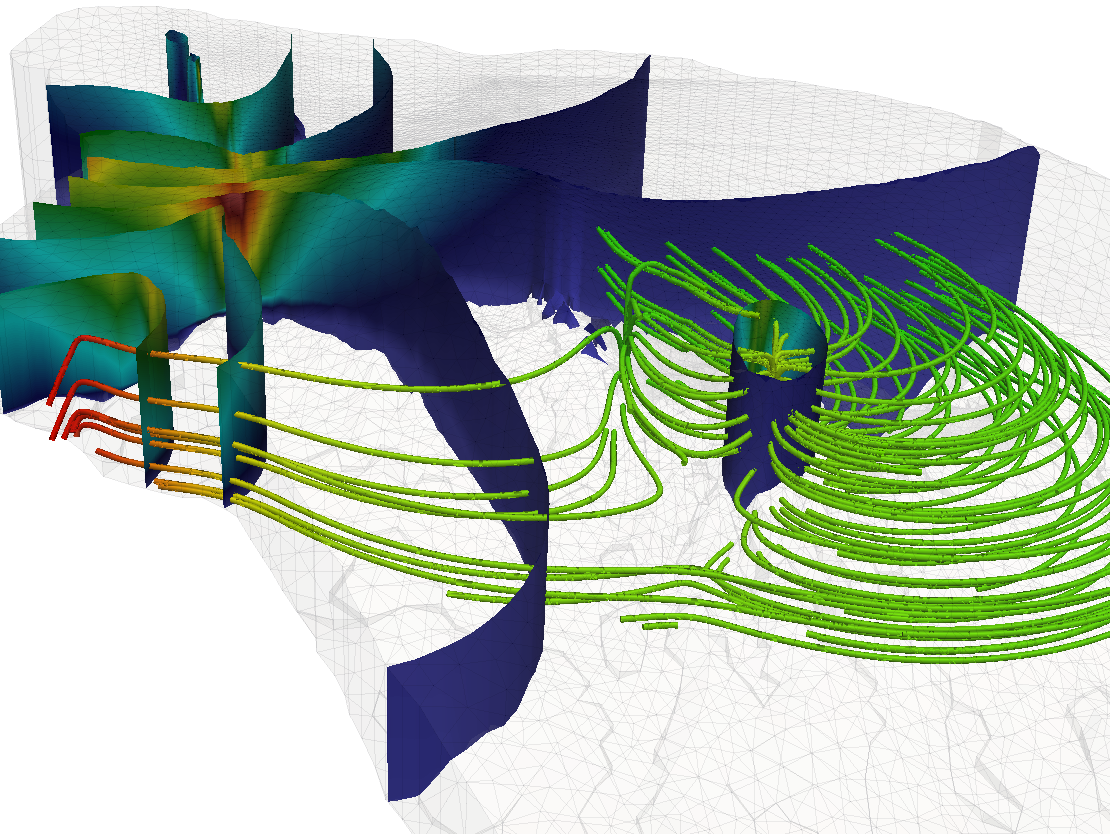
\includegraphics[width=0.48\linewidth]{ammer_sim.png}\label{fig:kr:ammer_sim}}
\end{center}
\caption{Visualization of data sets at various stages of the modeling process. (a) Input data from geographic information systems (GIS). (b) 3D surface model based on GIS data. (c) Subsurface model with layers interpolated based on borehole data. Different information is displayed for each geological layer. (d) Representation of simulation results using established visualization techniques such as isosurface and streamtracers.}
\label{fig:kr:vis}
\end{figure}

\subsection{Input Data}

As processes are simulated using the finite element method, adequate domain discretizations -- i.e. meshes -- need to be created either using the \emph{OpenGeoSys Data Explorer} or by employing other software.

For generating such a mesh using the \emph{Data Explorer}, geometric input data needs to be imported into the framework to define basic requirements such as the boundary of model region. This is done by selecting \cmd{File \ra Import files...} from the main menu and then selecting the appropriate file type. If external software has been employed, the corresponding mesh for the model region needs to be imported in a similar manner. The \emph{Data Explorer} supports a large number of established geo-scientific data formats, see figure \ref{fig:interfaces} for an overview. After selecting a specific file type, a file-open-dialogue will pop up and after choosing a file it is imported into the program.

If imported data will be needed again within \emph{OpenGeoSys} in the foreseeable future or if data has been somehow modified using the \emph{Data Explorer}, the respective data set should be saved to a native \emph{OpenGeoSys} file. To do this, the \emph{Data View} tab where the data set is listed (i.e. Geometry, Meshes, Stations or Modelling) needs to be selected and upon clicking the little disk-symbol on top of the tab the data will be saved. Geometric data will be written into a gml-file, meshes to vtu-files, station-data in stn-files and modelling data (i.e. Boundary conditions) in cnd-files. This process is repeated for every data set that needs to be converted and saved to an \emph{OpenGeoSys} format.

\begin{figure}[t]
\begin{center}
\subfloat[Feature embedding]{\frame{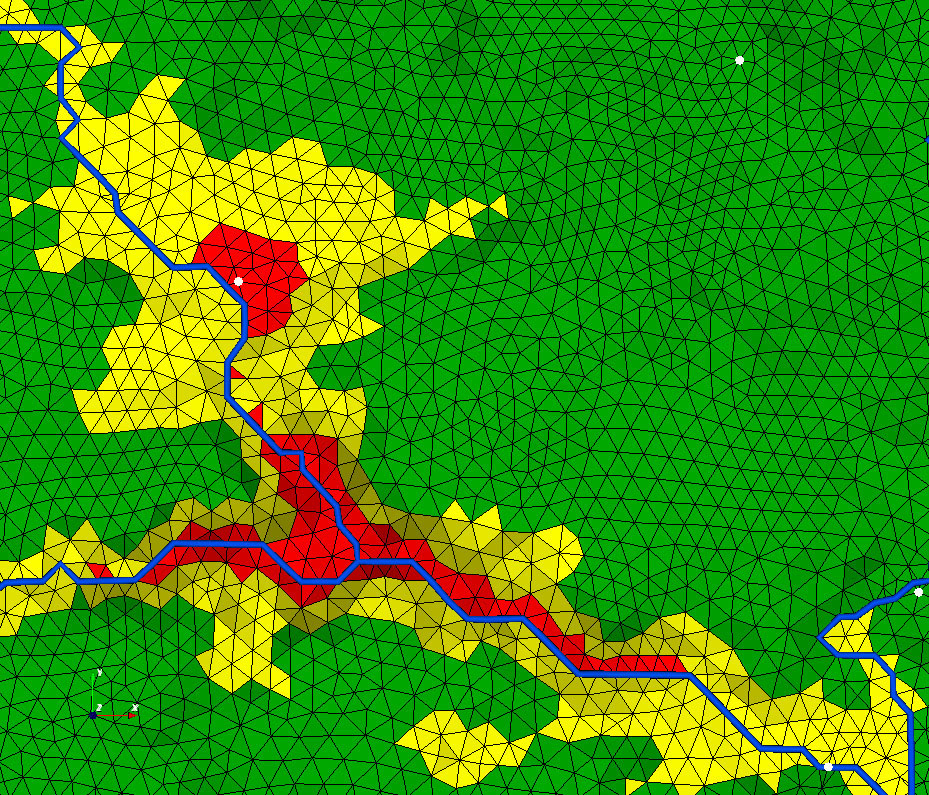
\includegraphics[width=.33\linewidth]{triangulation.png}}\label{fig:kr:triangulation}}\enspace
\subfloat[Mesh quality]{\frame{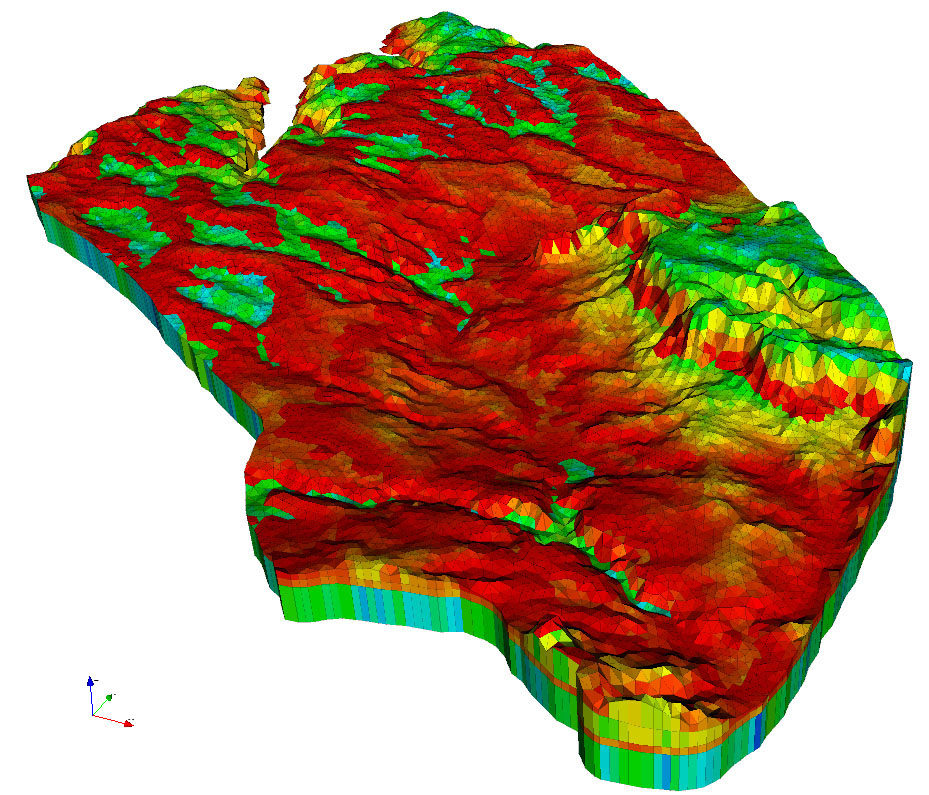
\includegraphics[width=.33\linewidth]{qual_edge_ratio.png}}\label{fig:kr:edgeratio}}\enspace
\subfloat[Element selection]{\frame{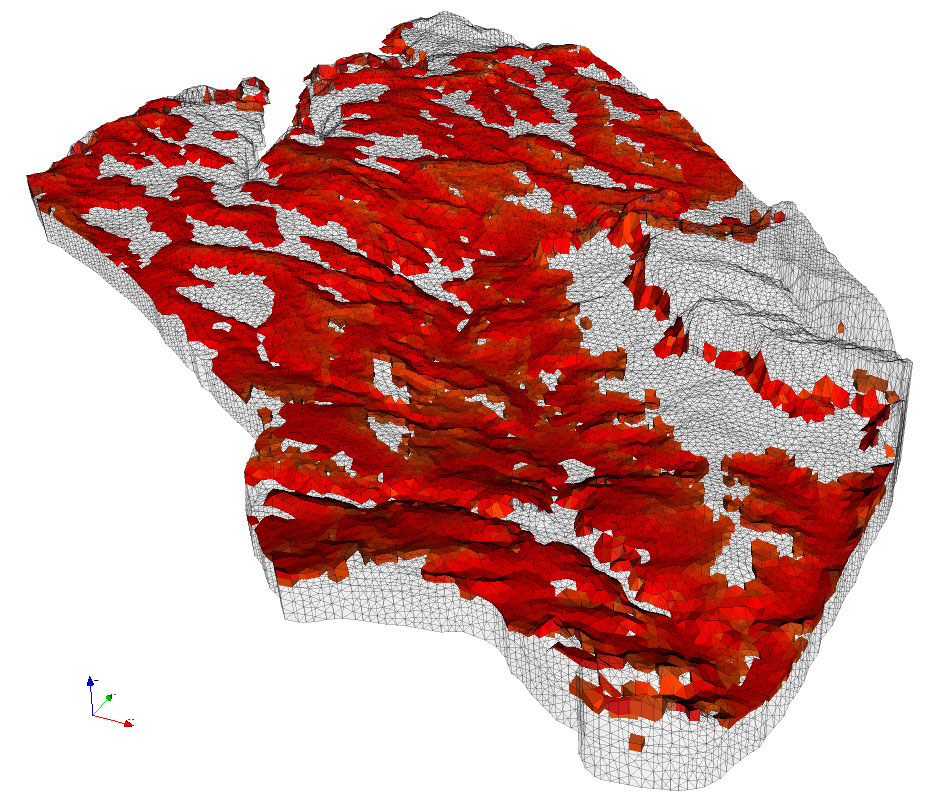
\includegraphics[width=.33\linewidth]{qual_edge_ratio_thresh.png}}\label{fig:kr:selection}}
\end{center}
\caption{Mesh quality validation: (a) Embedding geometric information representing rivers (blue) and wells (white) into the mesh structure. (b) Element quality based on edge ratio. Red/orange signifies large differences in edge length, green/blue signifies roughly equilateral elements. (c) Further analysis reveals that elements with a large edge ratio are the result of a thin surface layer.}
\label{fig:kr:meshqual}
\end{figure}

\subsection{Creating a 2D Surface Mesh}

The minimum requirements for creating a 2D mesh is a polygon representing the outer boundary of the model region as well as a digital elevation model (DEM) to derive the elevation at any point within the region (Fig.~\ref{fig:kr:ammer_gis}). Typically such data can be prepared using geographic information systems such as \emph{ArcGIS} but any supported data format will do.

In a first step, a triangulation of the area bounded by the polygon will be created. For detailed simulations, it is preferable to integrate additional data into the mesh that will be relevant for the model later on. Examples for this case study include the courses of rivers as well as a number of boreholes and wells. Boundary conditions will later be applied to these objects and integrating them into the mesh at the beginning of the model setup will ensure a less error-prone configuration of the model later on. See figure~\ref{fig:workflow:2Dmesh} for the effect of integrating these geometric objects when generating the mesh.
The process is started by selecting \cmd{Tools \ra Mesh Generation...} from the main menu. A dialog will open, where all data sets that have been loaded and might potentially be included into the new mesh are listed on the left hand side. By selecting data sets and moving them to the right hand side of the dialog they are added as constraints to be eventually included into the new mesh. When clicking on the \cmd{Advanced}-tab, a number of parameters for creating the mesh may be adjusted. Most importantly, the user can decide if the resulting mesh should have a homogeneous element size (all elements have roughly the same size as much as this is possible given the input data) or if the mesh should be adaptively refined towards geometrical features. This dialog also allows to change some weights employed by the meshing algorithm, with the general gist that smaller numbers will result in a finer mesh. 

When clicking \cmd{OK}, the 2D FEM mesh generator \emph{GMSH}~\cite{geuzaine:gmsh} is employed for creating
a 2D triangulation with elevation $z=0$ for all mesh nodes.

For a more detailed explanation on generating meshes from geometry, see section \ref{meshcreation}.

\begin{figure}[!h]
\begin{center}
\subfloat[Boundary only]{\includegraphics[width=0.3\linewidth]{ammer_geo1}}\enspace
\subfloat[With streams added]{\includegraphics[width=0.3\linewidth]{ammer_geo2}}\enspace
\subfloat[With boreholes added]{\includegraphics[width=0.3\linewidth]{ammer_geo3}}\\
\subfloat[Mesh from boundary]{\includegraphics[width=0.3\linewidth]{ammer_mesh1}}\enspace
\subfloat[Including streams]{\includegraphics[width=0.3\linewidth]{ammer_mesh2}\label{fig:ammer-mesh2}}\enspace
\subfloat[Including streams and boreholes]{\includegraphics[width=0.3\linewidth]{ammer_mesh3}\label{fig:ammer-mesh3}}\\
\subfloat[Mesh from boundary]{\includegraphics[width=0.3\linewidth]{ammer_meshgeo1}}\enspace
\subfloat[Including streams]{\includegraphics[width=0.3\linewidth]{ammer_meshgeo2}}\enspace
\subfloat[Including streams and boreholes]{\includegraphics[width=0.3\linewidth]{ammer_meshgeo3}}\\
\end{center}
\caption{Effect of adding information to the meshing process. The upper row shows geometric input data, with one data set added in each column. The resulting meshes are depicted in the second row. The meshes in figures~\ref{fig:ammer-mesh2} and \ref{fig:ammer-mesh3} have a similar refinement but in one mesh boreholes are located directly on mesh nodes and in the other mesh they are not. The bottom row gives a close-up of this effect to visualise how geometric information matches mesh nodes and edges if it has been integrated into the meshing process.\label{fig:workflow:2Dmesh}}
\end{figure}

In a second step, this coplanar mesh will be adjusted into an actual representation of the surface of the domain. This is done by mapping the elevation of mesh nodes based on an interpolation of the DEM of the region.  This can be done by right-clicking on the newly created 2D-mesh in the Mesh Data View and selecting \cmd{Edit mesh...}. When asked for the number of (subsurface) mesh layers, the input should be kept at $0$ since no subsurface layers need to be added at this stage. The dialog will then ask for the location of the DEM used for mapping and upon clicking \cmd{OK} the node elevations will be adjusted (Fig.~\ref{fig:kr:ammer_2d}). The DEM should cover the entire area enclosed by the polygon. For parts of the model area where no DEM information is available, a default value will be used. A triangulated representation of the surface area in the model region is created as a result and a visualization of this data set in 3D space is shown in the framework's render window. Further etails on that topic are given in section \ref{meshondemmapping}.


\subsection{Creating and Mapping Subsurface Layers}

Given the 2D mesh created in the last step, it is now possible to extrude this mesh into a 3D subsurface representation. Note that this surface need not necessarily be mapped based on DEM before creating a 3D mesh. However, performing the mapping step allows for a preliminary analysis of the surface and as such is a useful step for avoiding errors when applying other surface-related algorithms later on.

The 2D mesh should be right-clicked and \cmd{Edit mesh...} needs to be selected again. This time the number of desired subsurface layers needs to be entered before pressing \cmd{Next}.

There are two options for adding new layers to a 2D meshes:
\begin{enumerate}
\item Layers may have a constant thickness (although the thickness of different layers may vary)
\item Layer thickness may be based on elevation maps of subsurface layer boundaries in raster format (i.e. DEMs of layer boundaries, usually interpolated from borehole data)
\end{enumerate}

Depending on which option has been chosen, either the thickness of each layer has to be specified or, alternatively, the path to a DEM raster for each layer boundary needs to be selected.
In addition to layer boundaries, a DEM (i.e. Surface elevation) may be specified again, optionally. If a DEM is given, it will be used for cutting all information from interpolated layers that is located above the surface level specified in this file. This step might be necessary when using interpolated subsurface boundaries, to avoid the domain extending above the actual surface.

The dialog also allows to specify the type of domain discretization by offering the choice between creating prism or tetrahedra elements. Note that for the second option no actual 3D mesh is created. Instead, a 3D geometry for use in the open-source 3D FEM mesh generator \emph{TetGen}~\cite{tetgen:software} will be displayed as well as written into file. The result is a 3D mesh where each element has an ID indicating which material group (or layer) it belongs to (Fig.~\ref{fig:kr:ammer_3d}). Using the 3D visualisation of the \emph{Data Explorer} these different material groups will be displayed using different colors.

Note that subsurface layers can only be added to 2D meshes. Once layers have been added, the dimension of the mesh changes to 3D and adding additional layers automatically is no longer possible using the \emph{Data Explorer}.

Details on adding layers of fixed thickness can be found in section \ref{fixedsizelayers}, information for adding layers based on subsurface DEMs can be found in section \ref{meshondemmapping}.

\subsection{Quality Assurance}

Creating domain discretizations from complex input data might result in meshes containing suboptimal or even degenerated elements. While a lot of common sources of errors are automatically detected and, if possible, avoided, multiple complex datasets might still potentially result in a set of non-trivial geometric restrictions that will return incorrect or problematic results from the employed mesh generator. Therefore, the \emph{Data Expolorer} offers a set of algorithms for testing meshes for typical problems. A number of formal criteria are tested when selecting \cmd{Tools \ra Analyze Mesh...} from the main menu. After selecting the mesh to be tested and clicking \cmd{OK}, some obvious problems are automatically detected, including zero-volume-elements, non-convex elements, non-planar surfaces or nodes with a dangerously small distance between each other.

A visual representation of the quality of each mesh element can be creating by right-clicking on the mesh in the Data View and selecting \cmd{Calculate element quality...}. A meaningful criterium for the quality can be selected from a list, including typical metrics such as the ratio between shortest and longest edge in an element or the deviation of angles between edges from the optimum. As a result, mesh elements are colored using a heat-scale transfer function where blue indicates good element quality and red indicates bad element quality. An example is shown in figure~\ref{fig:kr:edgeratio}. In addition, a subset of elements can be chosen based on their quality. In figure~\ref{fig:kr:selection} only elements with an edge ration of $1:10$ or worse are displayed.

Using these algorithms, potential problems can at least be detected, if not automatically solved. Also, if and at what point an element will present a numerical problem during the simulation process can often not be decided in advanced. Different solvers or processes can be more or less restrictive given suboptimal conditions. Processes such as groundwater flow consist mainly of flows within a layered system, meaning that large differences between the extent of horizontal and vertical element surfaces might have no effect on the result. The simulation of mass transport processes explicitly requires a fine mesh resolution in vertical direction to ensure a stable solution. A more detailed discussion on the quality of mesh elements and their effect on simulation results can be found in literature \cite{knupp:quality, shewchuk:quality}.


%\section{Assigning FEM Conditions}
%
%conditions on geometrical objects
%
%setting conditions directly on meshes nodes


\section{Visualisation of Results}

If the output of simulation results is given in VTK-format, it is possible to load the files containing the results into the \emph{Data Explorer} via \cmd{Import files...\ra VTK}. Currently, time-steps have to be loaded seperately. Once loaded, all \ogs-visualisation options are available for manipulation of the result. This includes general visualisation options (detailed in section \ref{genvisoptions}) as well as visualisation filters (see section \ref{filters}).
The programme will automatically determine if the data loaded is a mesh or geometric data and will handle visualisation and filter options accordingly.


\appendix

\cleardoublepage
\addcontentsline{toc}{chapter}{Index}
\printindex

\cleardoublepage
\phantomsection
\addcontentsline{toc}{chapter}{Further Reading}

\begin{thebibliography}{}

\subsection*{OpenGeoSys Literature}

\bibitem{kalbacher:modelling}
Kalbacher T, Mettier R, et al.: Geometric modelling and object-oriented software concepts applied to a heterogeneous fractured network from the grimsel rock laboratory.
\emph{Comput Geosci,} \textbf{11(1):} 9--26 (2007)

\bibitem{kolditz:clean}
Kolditz O, Bauer S, Bilke L, et al.: OpenGeoSys: An open source initiative for numerical simulation of thermo-hydro-mechanical/chemical (THM/C) processes in porous media. \emph{Environ Earth Sci,} \textbf{67(2):}589--599 (2012)

\bibitem{kolditz:book}
Kolditz O, G�rke J-U, Shao H, Wang W (Eds): Thermo-Hydro-Mechanical-Chemical Processes in Fractured Media. Springer Berlin-Heidelberg, ISBN:978-3-642-27176-2, (2012)

\bibitem{ogs:web}
OpenGeoSys -- scientific software for coupled processes in porous media,
\texttt{http://www.opengeosys.org}

\bibitem{ogs:wiki}
OpenGeoSys-Wiki: Source code, current projects, presentations and much more. \texttt{https://svn.ufz.de/ogs/}

\bibitem{wang:thm}
Wang W, Kolditz O: Object-oriented finite element analysis of thermo-hydro-mechanical (THM) problems in porous media.
\emph{Int J Numer Meth Engng,} \textbf{69:}162--201 (2007)

\bibitem{wang:pfem}
Wang W, Kosakowski G, Kolditz O: A parallel finite element scheme for thermo-hydro-mechanical (THM) coupled problems in porous media \emph{Comput Geosci,} \textbf{35(8):}1631--1641 (2009)


\subsection*{Data Explorer Literature}

\bibitem{rink:envirvis}
Rink K, Bilke L, Kolditz O: Visualisation Strategies for Modelling and Simulation Using Geoscientific Data. \emph{Proc. of Workshop on Visualisation of Environmental Data, Leipzig Germany,} p. 47--51, The EuroGraphics Association.

\bibitem{rink:iemss}
Rink K, Bilke L, Selle B, Kolditz O: User Guided Generation of Hydrological Models: Interface Design, Workflows and Concepts for an Extensible Software Framework. \emph{Proc. of 6th
Int Congress on Environmental Modelling and Software (iEMSs2012), Leipzig, Germany,} (2012)

\bibitem{rink:modelcare}
Rink K, Fischer T, Gr�be A, Kolditz O: Visual Preparation of Hydrological Models. In \emph{Models -- Repositories of Knowledge,} IAHS Redbook \#355, ISBN: 978-1-907161-34-6, 113--118, (2012)

\bibitem{rink:cgvcvip}
Rink K, Fischer T, Kolditz O: Data Visualisation and Validation for Hydrological Models. \emph{Proc. of International Conference on Computer Graphics, Visualization, Computer Vision and Image Processing (CGVCVIP2011), Rome, Italy,} p. 169--176, (2011)

\bibitem{rink:catchres}
Rink K, Fischer T, Selle B, Kolditz O: A Data Exploration Framework for Validation and Setup of Hydrological Models.
\emph{Environ Earth Sci,} \textbf{69(2):}469--477, (2013)

\bibitem{rink:iwas}
Rink K, Kalbacher T, Kolditz O: Visual Data Exploration for Hydrological Analysis. \emph{Environ Earth Sci,} \textbf{65(5):} 1395--1403 (2012)


\subsection*{Case Studies}

\bibitem{gr�be:deadsea}
Gr�be A, R�diger T, Rink K, et al.: Numerical analysis of the groundwater regime in the western Dead Sea escarpment, Israel + West Bank. \emph{Environ Earth Sci,} \textbf{69(2):}571--585, (2013)

\bibitem{selle:wess}
Selle B, Rink K, Kolditz O: Recharge and discharge controls on groundwater travel times and flow paths to production wells for the Ammer catchment in SW Germany. \emph{Environ Earth Sci,} \textbf{69(2):}443--452, (2013)

\bibitem{sun:nankou}
Sun F, Shao H, Wang W, et al.: Groundwater deterioration in Nankou--a suburban area of Beijing: data assessment and remediation scenarios. \emph{Environ Earth Sci,} \textbf{67(6):}1573--1586, (2012)


\subsection*{Cited Literature}

\bibitem{knupp:quality}
P. M. Knupp: Achieving finite element mesh quality via optimization of the Jacobian matrix norm and associated quantities. Part I--a framework for surface mesh optimization. \emph{Int J Numer Meth Eng,} \textbf{48:}401--420, (2000)

\bibitem{shewchuk:quality}
J. R. Shewchuk: What is a Good Linear Finite Element? Interpolation, Conditioning, Anisotropy, and Quality Measures. \emph{Department of Electrical Engineering and Computer Science, University of Berkeley,} (2002)

\bibitem{tetgen:software}
H. Si: TetGen -- A Quality Tetrahedral Mesh Generator and Three-Dimensional Delaunay Triangulator. \emph{WIAS Technical Report No. 13,} Weierstrass Institute for Applied Analysis and Stochastics, (2013) \\
\url{http://www.tetgen.org}

\bibitem{geuzaine:gmsh}
C. Geuzaine and J.-F. Remacle: Gmsh: a three-dimensional finite element mesh generator with built-in pre- and post-processing facilities. \emph{Int J Numer Meth Eng,} \textbf{79(11):}1309--1331, (2009) \\
\url{http://geuz.org/gmsh}

\end{thebibliography} 

\cleardoublepage

\end{document}
